\section{Background Subtraction}
\label{sec:BackgroundSubtraction}

In the selected sample we have our signal events as well as event coming from various background. To compute cross section, we need to subtract background and estimate how many events in each $P_T^\gamma$ bin originate from the $W\gamma$ process. This chapter describes the methods used for the background subtraction and provides plots and tables with the results.

\subsection{Fake Photon (from Jets) background estimation and subtraction}
\label{sec:BackgroundSubtraction_jtog}

After passing through all selection criteria, the selected sample is dominated by $W$+jets background and this background cannot be further significantly reduced without reducing our signal sample $W\gamma$ as well. The photon ID helps to reduce $W$+jets to a certain level but there is still a significant number of jets which are reconstructed as photons and pass all the photon ID criteria. DY+jets is another source of jets$\rightarrow \gamma$ background but this one is significantly suppressed by $M_W^T$ cut in both channels and by the $Z$-mass window cut in the electron channel.

The template method is used to estimate jets$ \rightarrow \gamma$ background. The method requires real-$\gamma$ template ($T_{true}$) and fake-$\gamma$ template ($T_{fake}$). Then the fit is performed according to: 
\begin{equation}
F(V_{fit})=N_{true} \cdot T_{true}(V_{fit}) + N_{fake} \cdot T_{fake}(V_{fit}),
\end{equation}
\noident{where $V_{fit}$ is a fit variable, $N_{true}$ and $N_{fake}$ are numbers of real and fake photons in the data sample respectively.}

% EXPLAIN WHAT IS I_{CH}^{\gamma} and WHAT IS SIHIH
We use $V_{fit}=I_{ch}^{\gamma}$ and $V_{fit}=\sigma_{i\eta i\eta}^{\gamma}$. To prepare templates, we use $Z\gamma$-selected dataset. Real-$\gamma$ templates $T_{true}$ are taken from the FSR-selected events of $Z\gamma\rightarrow\mu\mu\gamma$ while fake-$\gamma$ templates are taken from the $Z\gamma$(ISR)-selected dataset.

The FSR $Z\gamma$ selection has looser $\Delta R_{min}(\mu,\gamma)$ cut of $\Delta R_{min}(\mu,\gamma)>0.4$ (while the nominal cut is $\Delta R_{min}(\mu,\gamma)>0.7$) and has three-particle invariant mass cut $M_{\gamma\mu\mu}<101$~GeV. The FSR sample does not have enough number of events for high $P_{T}^{\gamma}$ bins but the distribution of $I_{ch}^{\gamma}$ of real photons does not depend on $P_{T}^{\gamma}$ and, therefore, events for $P_{T}^{\gamma}>15~GeV$ are all merged to prepare templates. Distributions of $\sigma_{i\eta i\eta}^{\gamma}$ do depend on $P_T^{\gamma}$. Only events of $P_T^{\gamma}>30~GeV$ are merged together to prepare templates for all $P_T^{\gamma}>30~GeV$ bins. Templates for barrel and endcap photons are prepared separately.

$Z\gamma$(ISR)-selected dataset consists of $Z\gamma$+DYjets events. DY+jets events are needed to construct a fake photon template. Non-negligible real-$\gamma$ contribution is subtracted using $Z\gamma$ MC predictions. ISR events were selected using nominal $Z\gamma$ selection and $M_{ll\gamma}>101$~GeV, $\Delta{R_{min}}(\mu,\gamma)>1.0$ cuts. 

FSR and ISR selections are illustrated in App.~\ref{sec:ZgFSRandISRplots}. Distributions of $M_{ll\gamma}$ and $M_{ll}$ for nominally selected $Z\gamma$ dataset are shown in Fig.~\ref{fig:Zg_Mleplep_and_Mpholeplep}. Distributions of $\Delta{R}(l,\gamma)$ for ISR and FSR $Z\gamma$ events are shown in Fig.~\ref{fig:Zg_ISRandFSR_dR}. Distributions of $P_{T}^{\gamma}$ for ISR and FSR $Z\gamma$ events are shown in Fig.~\ref{fig:Zg_ISRandFSR_phoEt}. High $P_{T}^{\gamma}$ bins have higher real-$\gamma$ contamination but even the very last bin has large enough number of events to prepare a template. 

The $P_{T}^{\gamma}$ dependence of the real-$\gamma$ and fake-$\gamma$ templates are shown in Fig.~\ref{fig:compareTemplatesTruePtDep}-\ref{fig:compareTemplatesFakePtDep} in the App.~\ref{sec:CompareTemplatesPlots}. 

The real-$\gamma$ and fake-$\gamma$ templates are the same for muon and electron channels. Fig.~\ref{fig:compareTemplatesTruePtDep}-\ref{fig:compareTemplatesFakePtDep} demonstrate that real-$\gamma$ templates are not $P_{T}^{\gamma}$ dependent while fake-$\gamma$ templates are.

To extract real-$\gamma$ yield from the $N_{true}$, efficiency of the $V_{fit}$ is applied on the value derived from fit based on the distribution of events which are used to prepare the real-$\gamma$ template. To extract fake-$\gamma$ yield from the $N_{fake}$, efficiency of the $V_{fit}$ is applied on the value derived from fit based on the distribution of events which are used to prepare a fake-$\gamma$ template. Plots of the template fits are available in App.~\ref{sec:TemplateFitPlots} for fits on data. 

Several cross checks are performed to validate the procedure. Two MC closure checks are performed to validate the procedure. For the first check all MC samples that pass $W\gamma$ selection are mixed together with appropriate weights assigned. Then fits on this sample of pseudodata is performed as on real data and the fit results are superimposed with MC samples. The results of the MC closure check are reported in App.~\ref{sec:MCclosureCheck} and the fit plots are shown in App.~\ref{sec:TemplateFitPlotsMCclosure}. 

For the second MC-closure check, the pseudodata sample is prepared from $W$+jets and $W\gamma$ samples only. The results are reported in App.~\ref{sec:TemplateFitPlotsMCclosureWjetsPlusWg}. 

\subsection{Fake Photon (from Electron) Data Driven Background for Electron Channel}
\label{sec:BackgroundSubtraction_etog}

For the electron channel, DYjets is the main source of the $e \rightarrow \gamma$ background. The $Z$-mass window cut of $70$~GeV$<M_{e\gamma}<110$~GeV significantly suppresses this background, however, the remaining contribution is non-negligible. 

Data-driven contribution of $e\rightarrow\gamma$ is estimated separately for each $P_{T}^{\gamma}$ bin and separately for barrel and endcap using the following expression: $N_{data-nom}^{e\rightarrow\gamma} = N_{MC-nom}^{e\rightarrow\gamma} \cdot N_{data-Zpeak}^{e\rightarrow\gamma}/N_{MC-Zpeak}^{e\rightarrow\gamma}$. 

\begin{itemize}
  \item Get $N_{MC-Zpeak}^{e\rightarrow\gamma}$ (number of $e\rightarrow\gamma$ events under the $Z$-peak based on the MC prediction); done by counting
  \item Get $N_{data-Zpeak}^{e\rightarrow\gamma}$ (number of $e\rightarrow\gamma$ events under the $Z$-peak from data); done by fitting; all other cuts to prepare the dataset are applied
  \item Get $N_{MC-nom}^{e\rightarrow\gamma}$ (number of $e\rightarrow\gamma$ events in the nominal range based on the MC prediction); done by counting
  \item Get $N_{data-nom}^{e\rightarrow\gamma}$ (number of $e\rightarrow\gamma$ events in the nominal range based on the MC predictionfrom data); done by scaling $N_{data-nom}^{e\rightarrow\gamma} = N_{MC-nom}^{e\rightarrow\gamma} \cdot N_{data-Zpeak}^{e\rightarrow\gamma}/N_{MC-Zpeak}^{e\rightarrow\gamma}$
\end{itemize}

The number of $e\righarrow\gamma$ events in data under the $Z$-peak $N_{MC-Zpeak}^{e\rightarrow\gamma}$ is extracted from the fit of the model: $N_{sig} \cdot (RooNDKeysPdf~x~Gaussian) +  N_{bkg} \cdot (RooCMSShapePdf)$. The fits are performed separately in ech $P_T^\gamma$ bin in fine $\eta^\gamma$ binning:
     \begin{itemize}
        \item $P_T^\gamma$ 15-20-25-30-35-45-55-65 GeV
           \begin{itemize}
              \item $\eta^\gamma$ binning in barrel: 0.00-0.10-0.50-1.00-1.44
              \item $\eta^\gamma$ binning in endcap: 1.56-2.10-2.20-2.40-2.50
           \end{itemize}
        \item $P_T^\gamma$ 65-75-85-95 GeV
          \begin{itemize}
              \item $\eta^\gamma$ binning in barrel: 0.00-0.50-1.44
              \item $\eta^\gamma$ binning in endcap: 1.56-2.20-2.50
           \end{itemize}
        \item $P_T^\gamma$: 95-120-500 GeV
          \begin{itemize}
              \item $\eta^\gamma$ binning in barrel: 0.00-1.44
              \item e$\eta^\gamma$ binning in ndcap: 1.56-2.50
           \end{itemize}
        \item $P_T^\gamma$ 10-15 GeV (underflow bin): MC-prediction is used, no fit performed.
     \end{itemize}
\noident{The fit plots are provided in App.~\ref{sec:EtogammaFitPlots} and the tables are provided in App.~\ref{sec:etogTables}. To prepare yields, fit results in all fine barrel $\eta^\gamma$ bins are summed up and fit results in all fine endcap $\eta^\gamma$ bins are summed up. The distributions of $M_{e\gamma}$ before and after appropriate scale of the $e\rightarrow\gamma$ of the DY+jets sample is in different $P_T^{\gamma}$ bins are shown in App.~\ref{sec:Mpholep1DatavsMC}.}

%  \item templates for RooNDKeysPdf: $e\rightarrow\gamma$ portion of the DYjets MC separately for each pt-eta bin
%  \item $e\rightarrow\gamma$ portion of the DYjets MC: a photon has a gen-level electron within dR=0.4 







\subsection{Other Backgrounds}

In addition to the backgrounds discussed before, there are several more sources:
\begin{itemize}
   \item real-$\gamma$ background. Main sources of the real-$\gamma$ background are Z$\gamma$ and W$\gamma \rightarrow \tau \nu \gamma$. The MC-based estimation is used to subtract these backgrounds.
   \item The $e \rightarrow \gamma$ background for muon channel. Sources of these backgrounds are $WW$ ($W \rightarrow \mu\nu_{\mu}$ + $W \rightarrow e\nu_e$), $WZ$ ($W \rightarrow \mu\nu_{\mu}$ + $Z \rightarrow ee$ or $W \rightarrow e\nu_{\mu}$ + $Z \rightarrow \mu\mu$) and $ZZ$ ($Z \rightarrow \mu\mu$ + $Z \rightarrow ee$). This background is neglected.
   \item Jets$ \rightarrow $lepton + real-$\gamma$ ($\gamma$+jets and $\gamma\gamma$+jets events). Neglected.
   \item Jets$ \rightarrow $lepton + jets$ \rightarrow \gamma$. Neglected. 
\end{itemize}
\noindent{The neglected backgrounds were studied based on their MC samples in the muon channel. The total contribution of $WW$+$WZ$+$ZZ$+($\gamma\gamma$+jets)+($\gamma$+jets)+$W\gamma \rightarrow \tau\nu_{\tau}\gamma$ without $M_T^W$ cut in the muon channel was found to be~\~2.2\% of the total MC and~\~8\% of $W\gamma \rightarrow \mu\nu_{\mu}\gamma$. In the samples ($\gamma\gamma$+jets) and ($\gamma+jets$) almost no events passed the selection criteria. $WW$, $WZ$ and $ZZ$ contributions are shown to be negligible compared to $W\gamma \rightarrow \tau\nu_{\tau}\gamma$ and $WW\gamma$ and are not shown at the plots too.}



\subsection{$P_T^{\gamma}$ Spectrum, Signal and Background}

\begin{figure}[htb]
  \begin{center}
   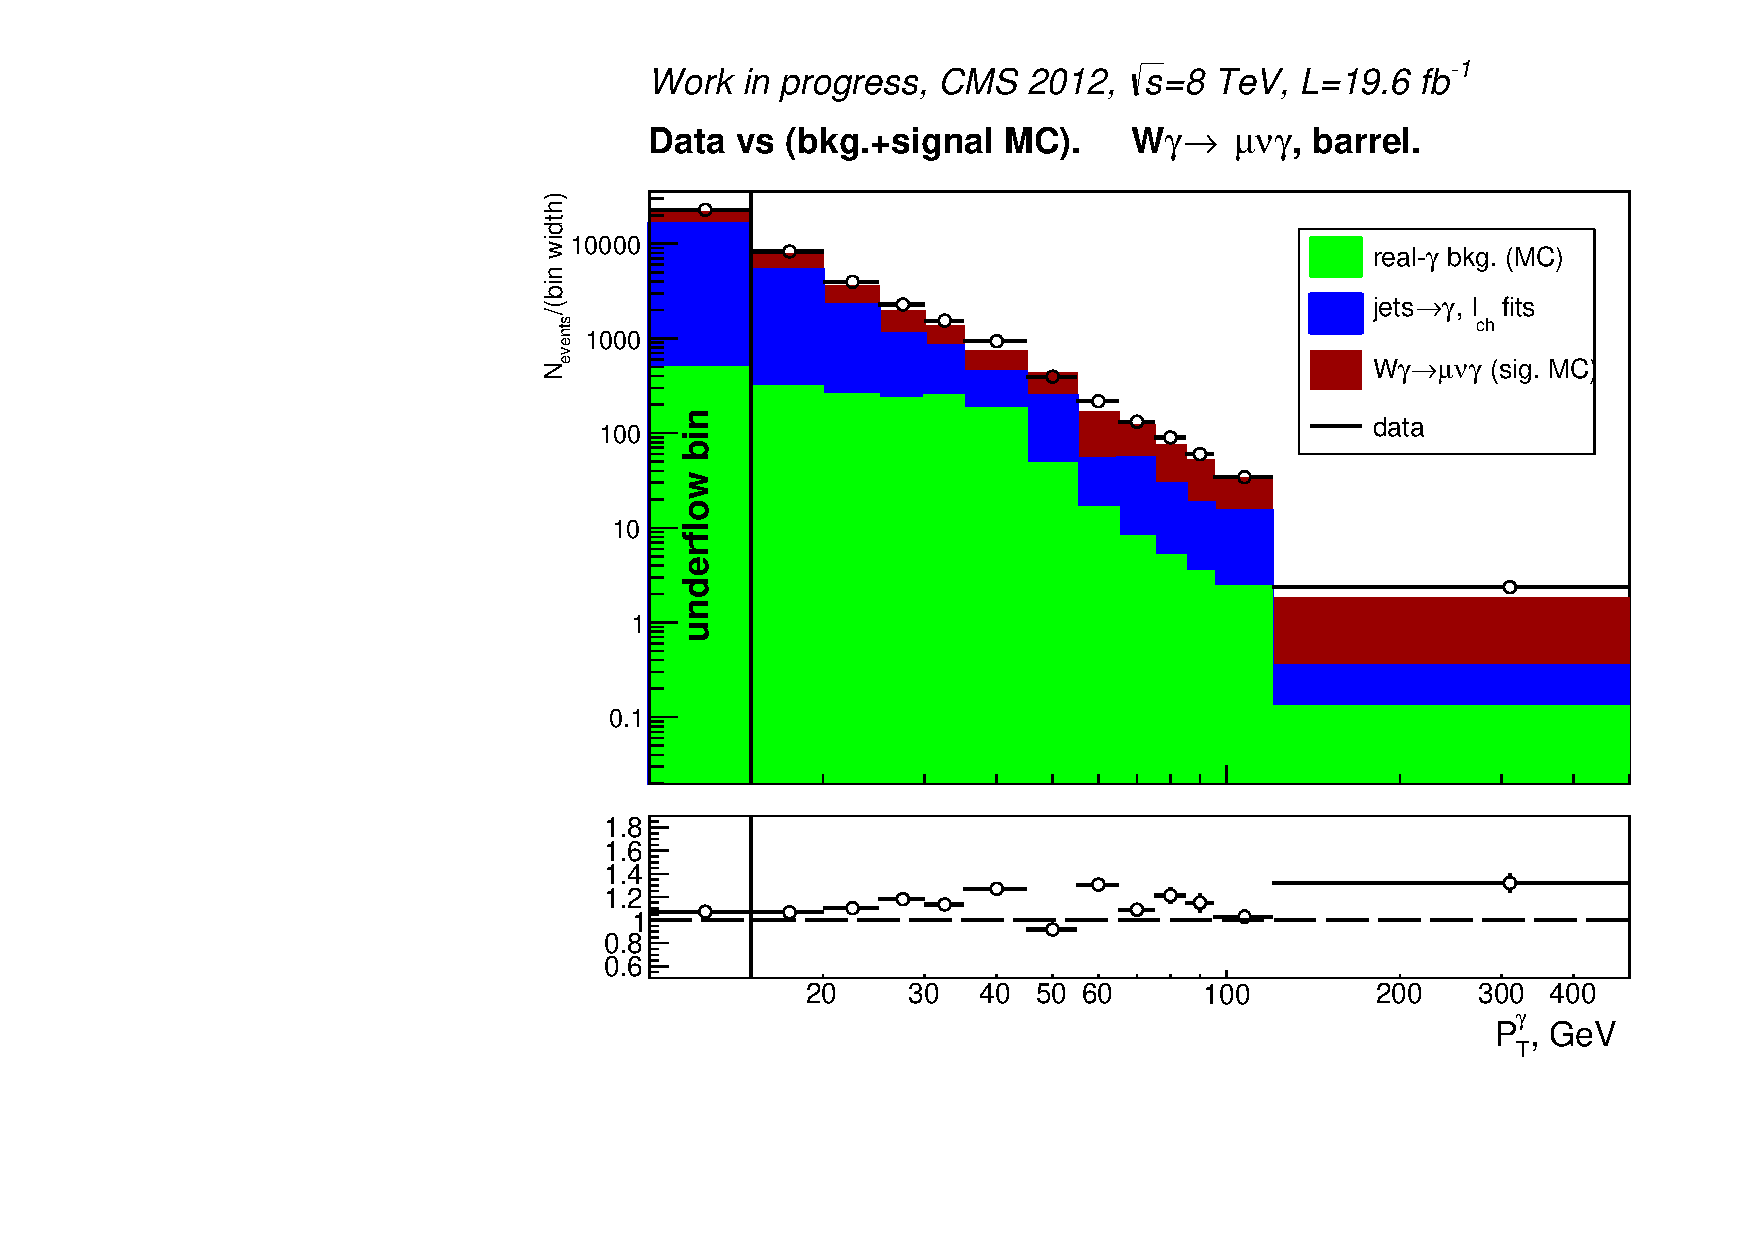
\includegraphics[width=0.45\textwidth]{../figs/figs_v11/MUON_WGamma/PrepareYields/c_DATAvsBkgPlusSigMCc_MUON_WGamma_TEMPL_CHISO_UNblind__Barrel__phoEt.pdf}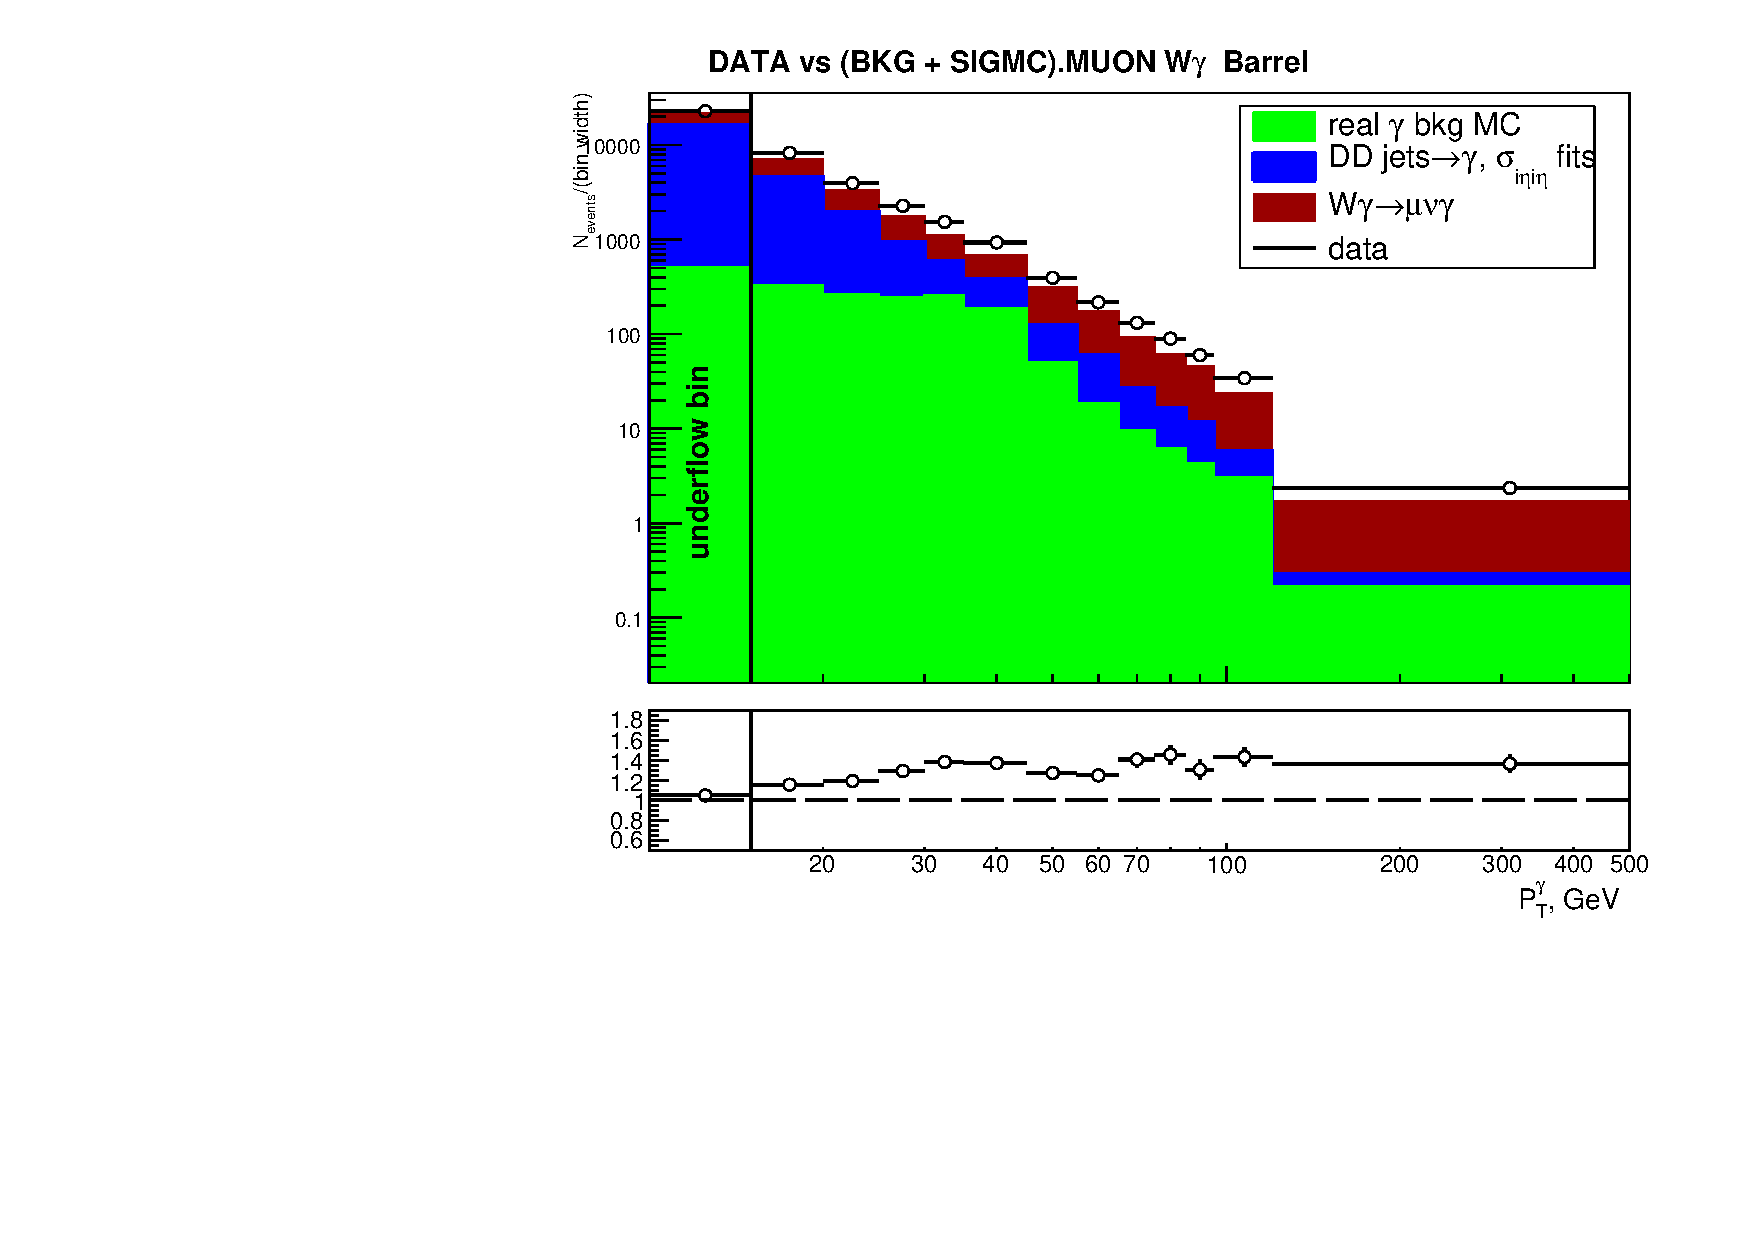
\includegraphics[width=0.45\textwidth]{../figs/figs_v11/MUON_WGamma/PrepareYields/c_DATAvsBkgPlusSigMCc_MUON_WGamma_TEMPL_SIHIH_UNblind__Barrel__phoEt.pdf}  \\
   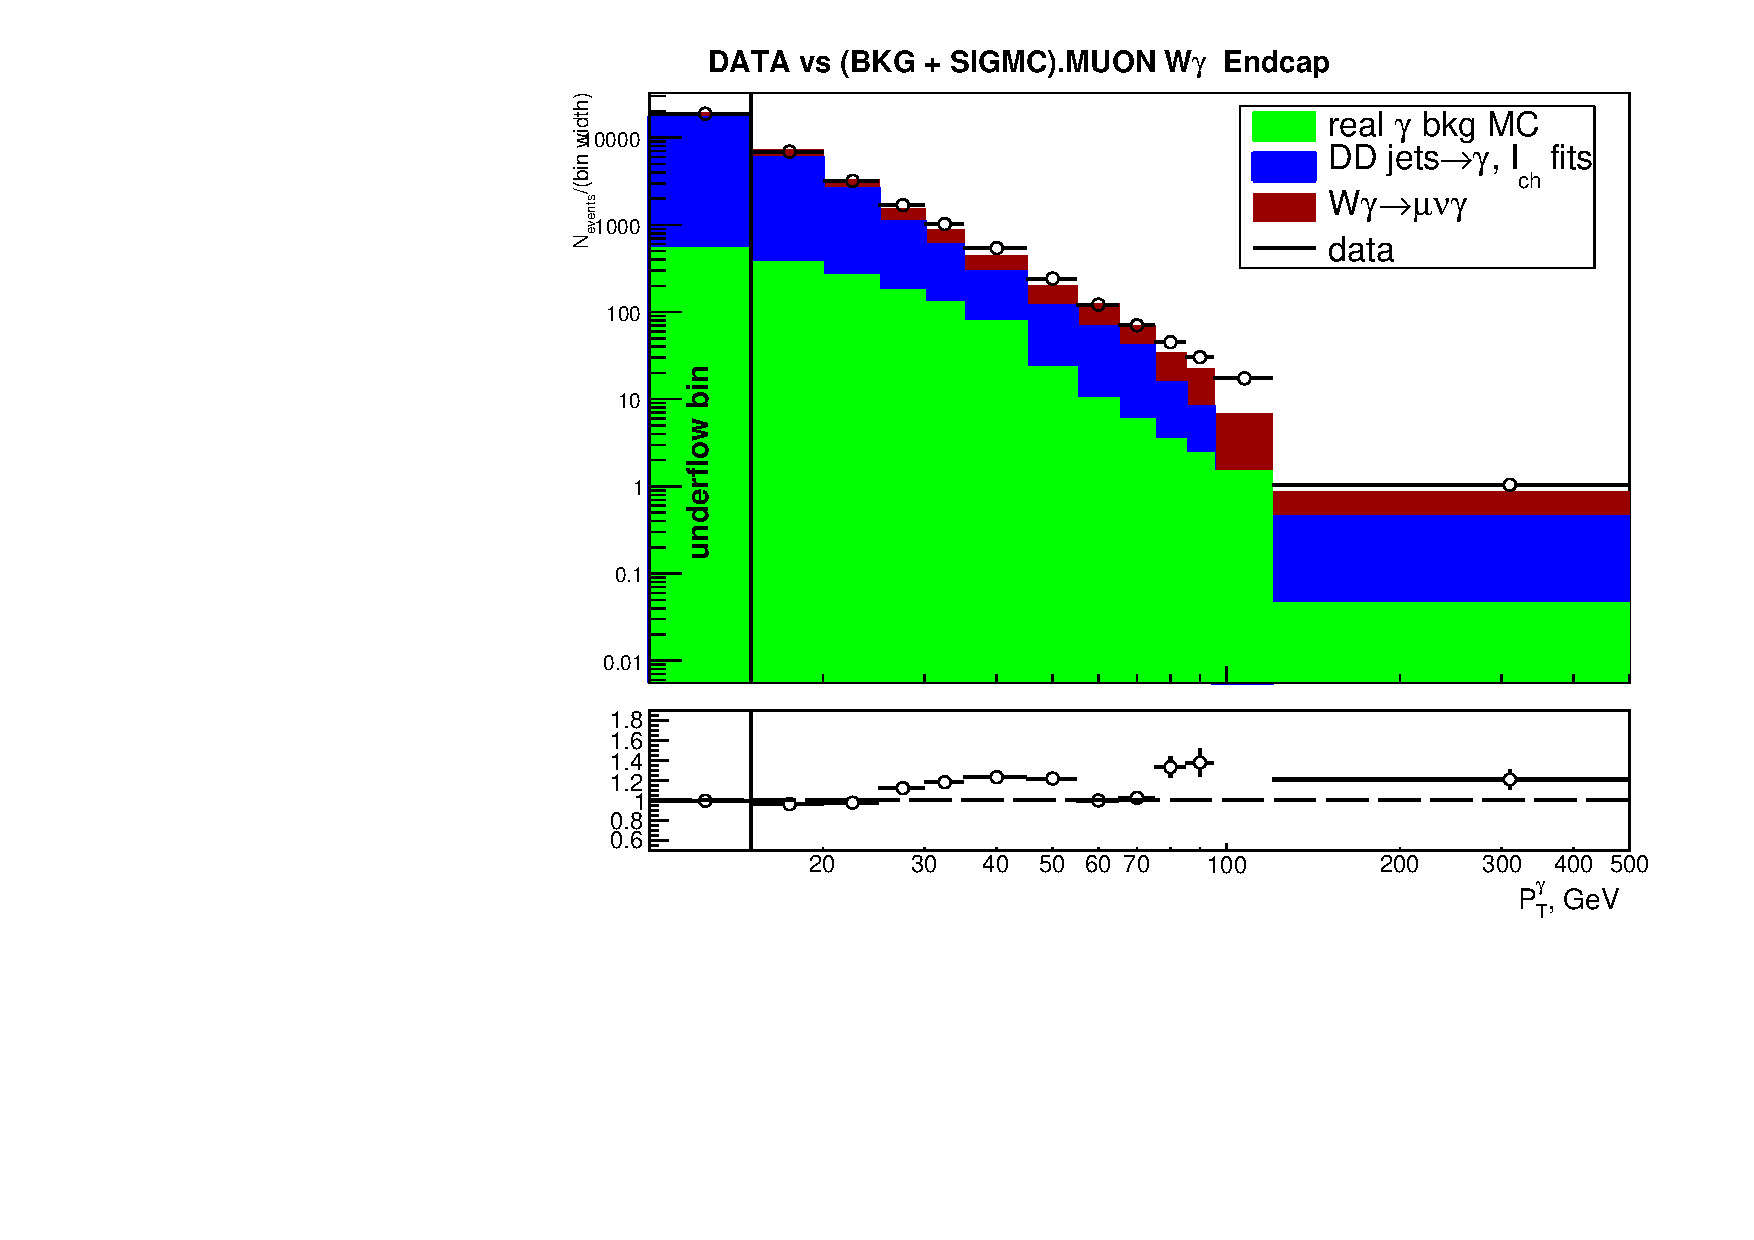
\includegraphics[width=0.45\textwidth]{../figs/figs_v11/MUON_WGamma/PrepareYields/c_DATAvsBkgPlusSigMCc_MUON_WGamma_TEMPL_CHISO_UNblind__Endcap__phoEt.pdf}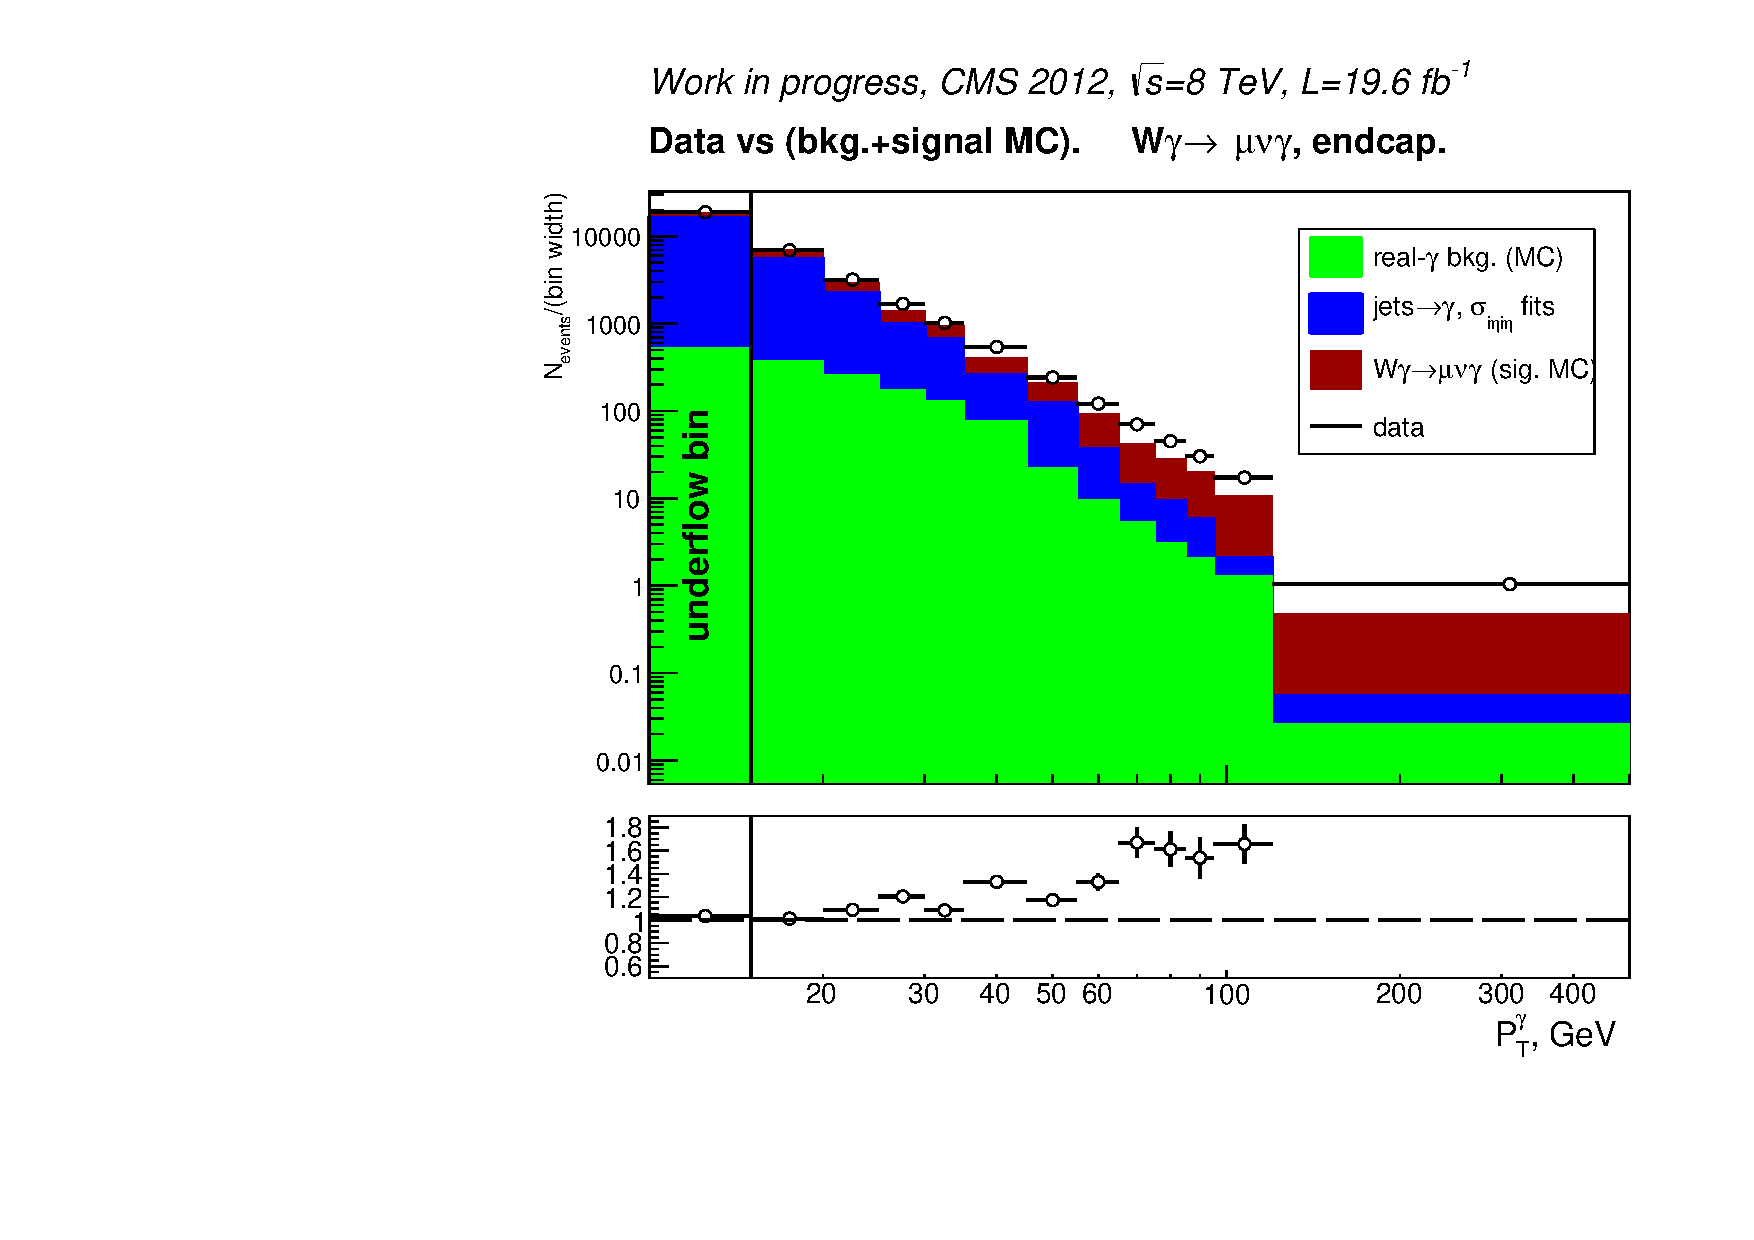
\includegraphics[width=0.45\textwidth]{../figs/figs_v11/MUON_WGamma/PrepareYields/c_DATAvsBkgPlusSigMCc_MUON_WGamma_TEMPL_SIHIH_UNblind__Endcap__phoEt.pdf}  \\
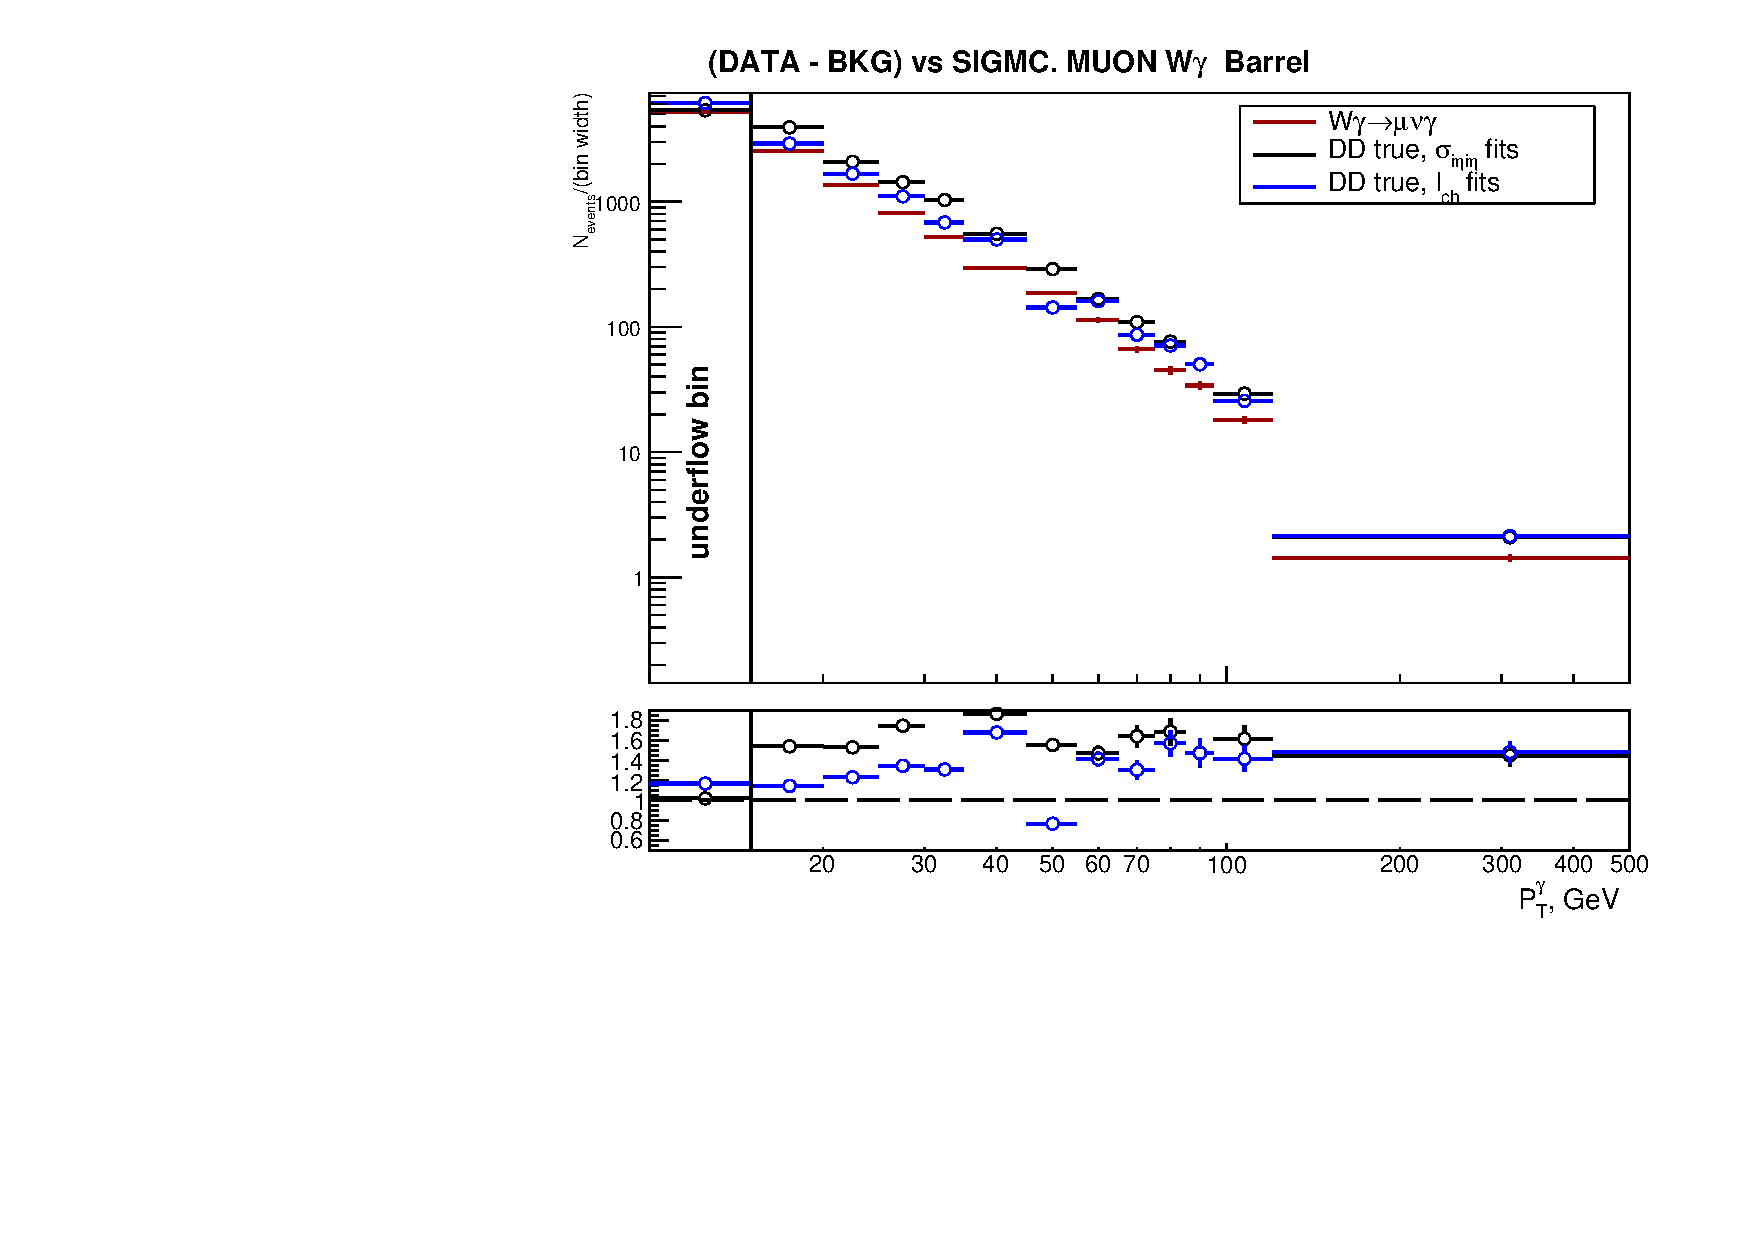
\includegraphics[width=0.45\textwidth]{../figs/figs_v11/MUON_WGamma/PrepareYields/c_BkgSubtrDATAvsSIGMC_c_MUON_WGamma__UNblind__Barrel__phoEt.pdf}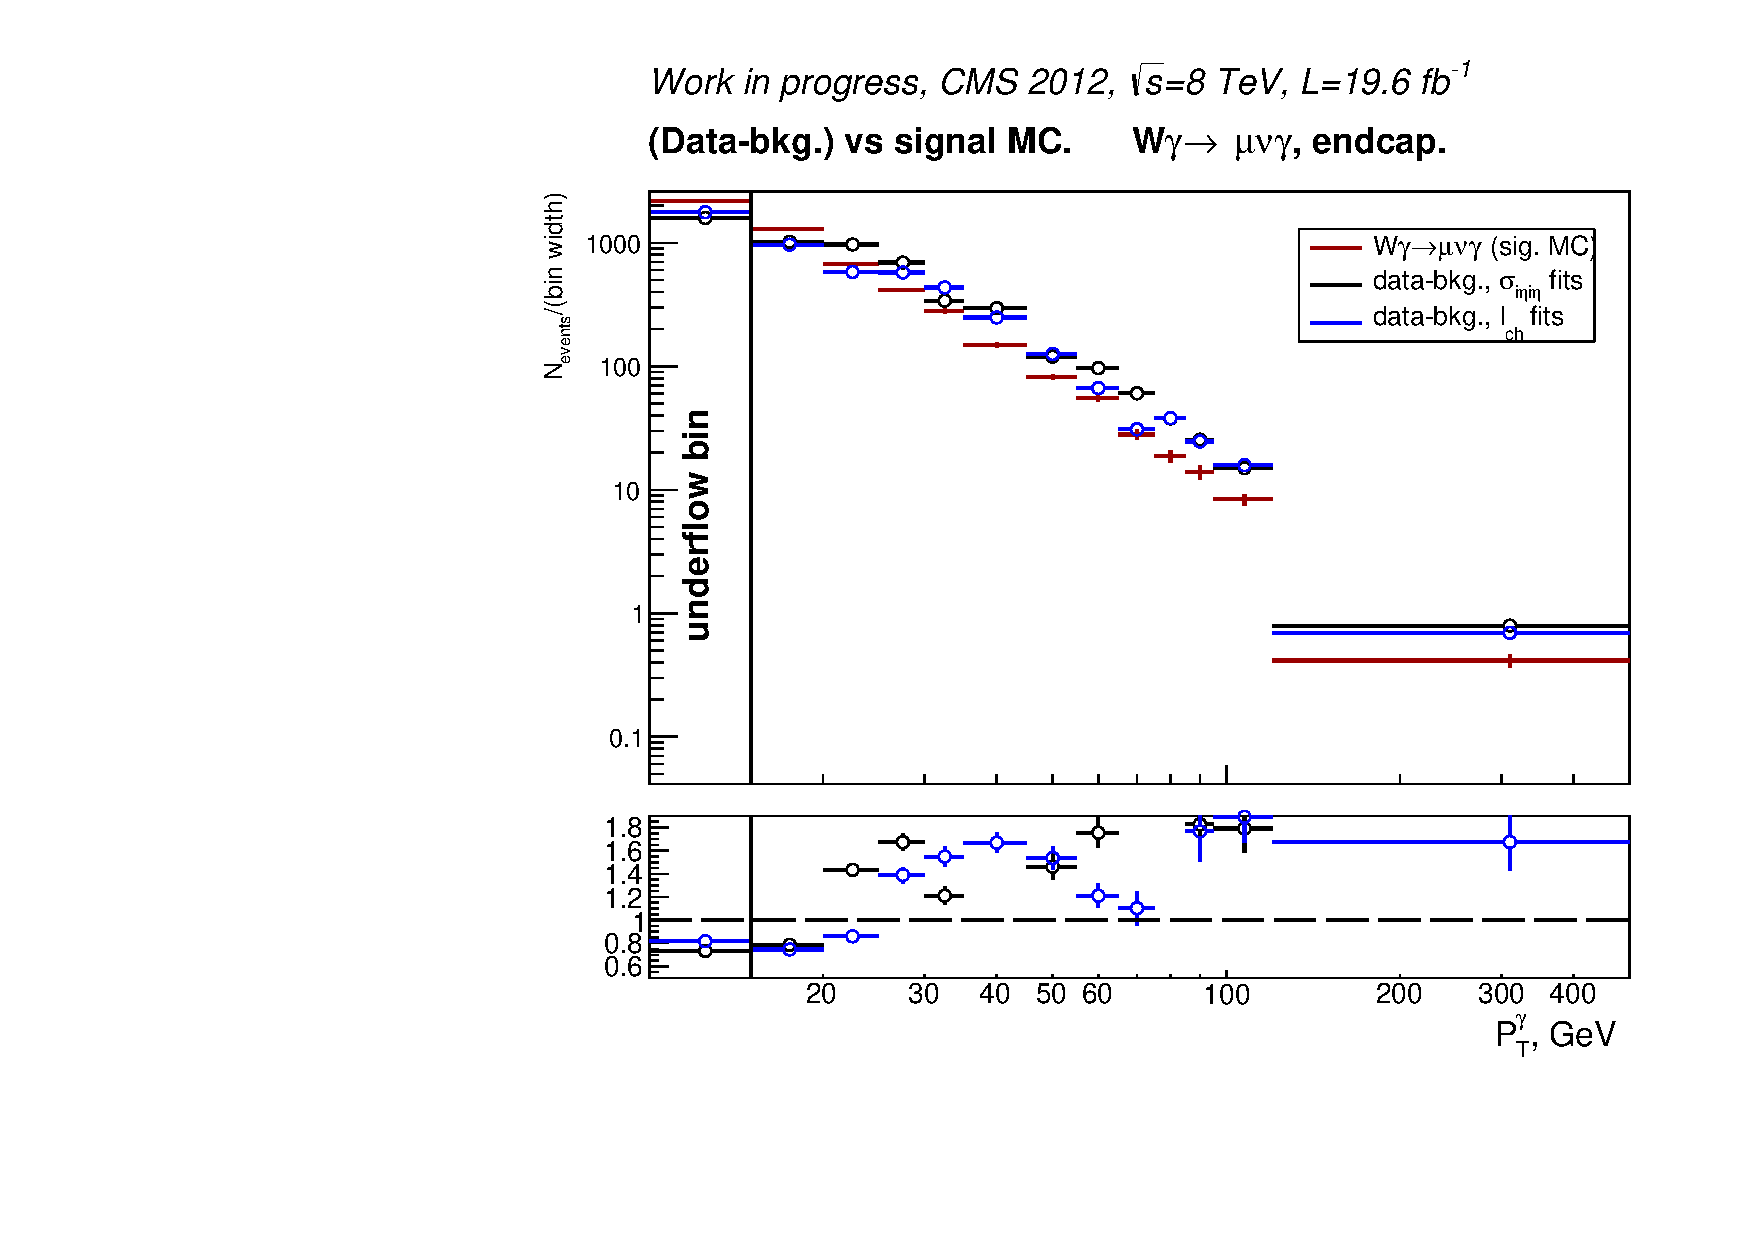
\includegraphics[width=0.45\textwidth]{../figs/figs_v11/MUON_WGamma/PrepareYields/c_BkgSubtrDATAvsSIGMC_c_MUON_WGamma__UNblind__Endcap__phoEt.pdf}\\
  \caption{Top and middle: data vs fake-$\gamma$ background derived from the template method + real-$\gamma$ background predicted by dedicated MC samples + signal MC, with $I_{ch}$ and $\sigma_{i\etai\eta}$ used as fit variables. Bottom: data yields after full background subtraction vs signal MC. $I_{ch}$ vs $\sigma_{i\etai\eta}$ fit results. }
  \label{fig:DDvsMC_Wg_Data_MUON}
  \end{center}
\end{figure}

\begin{figure}[htb]
  \begin{center}
   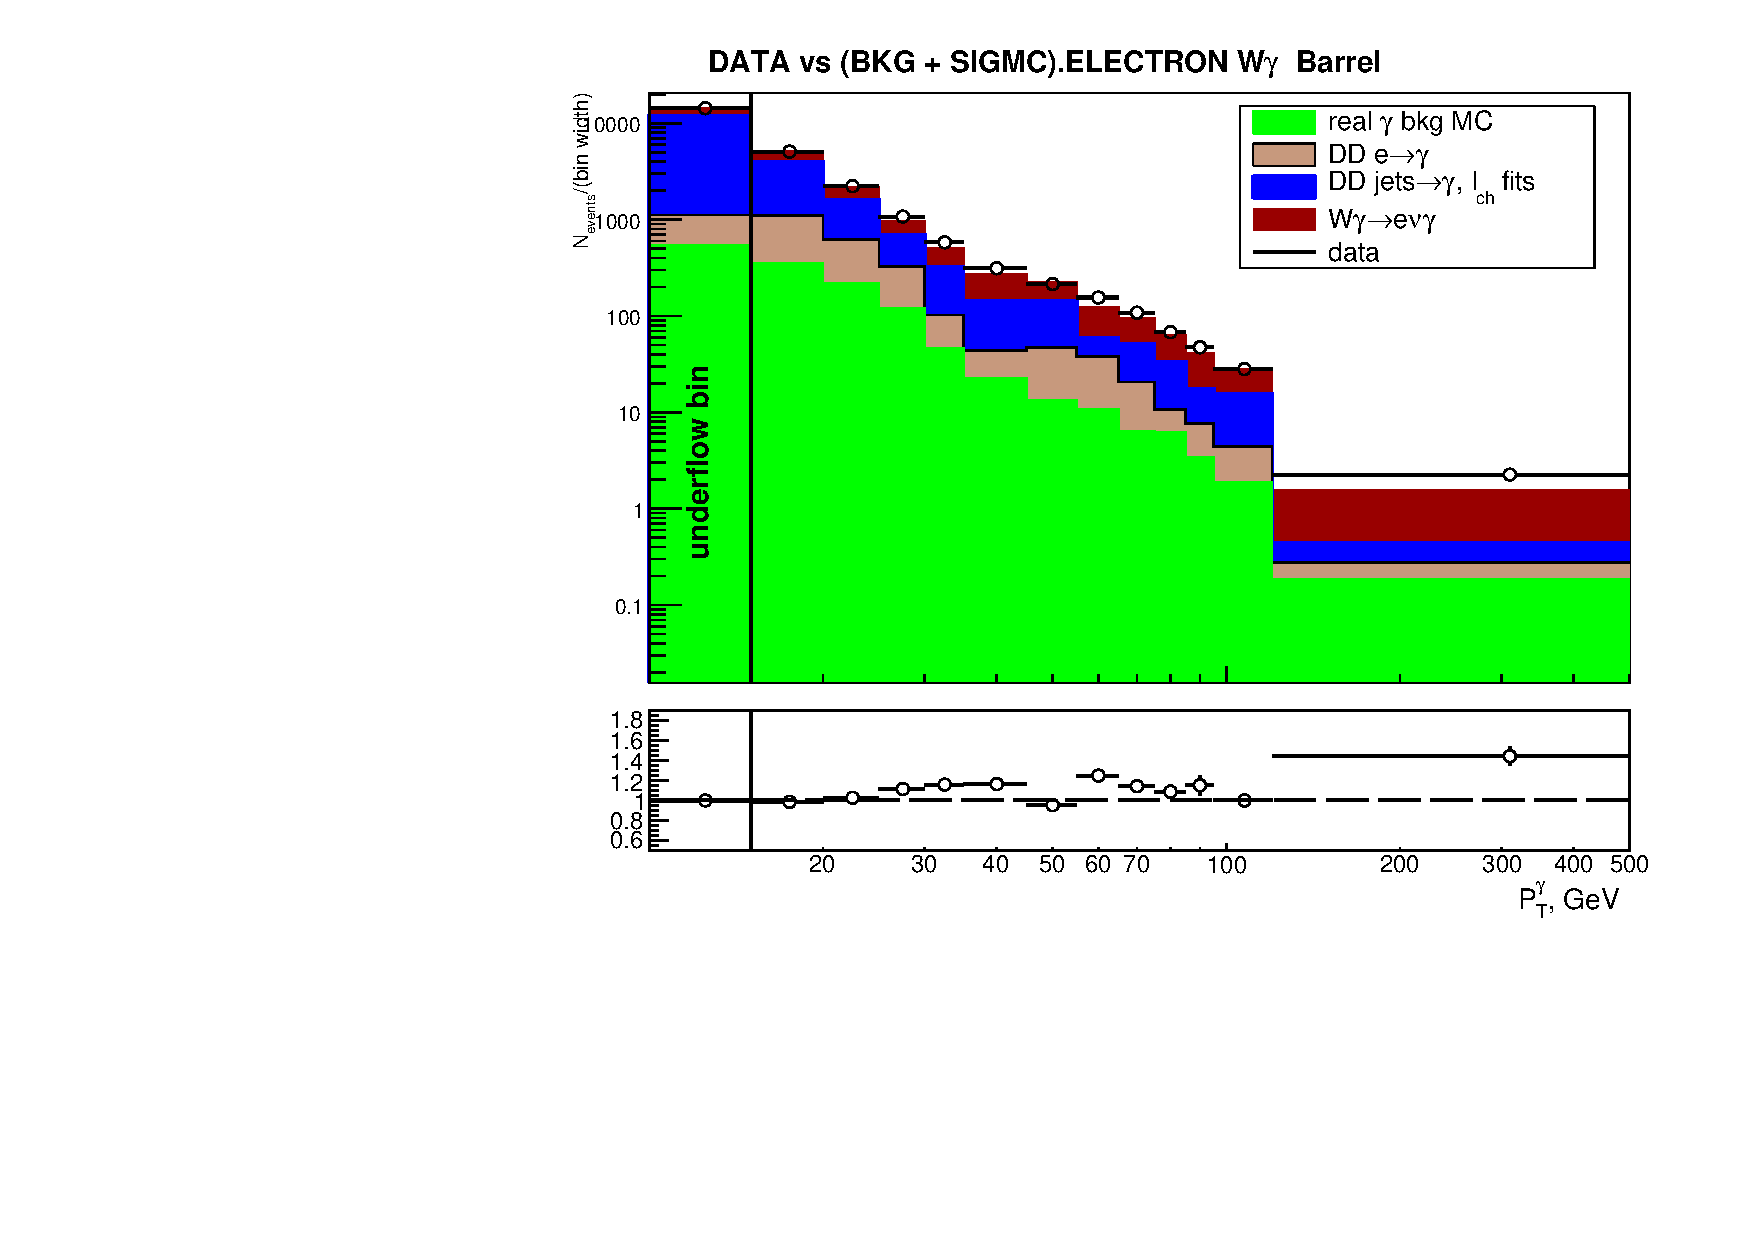
\includegraphics[width=0.45\textwidth]{../figs/figs_v11/ELECTRON_WGamma/PrepareYields/c_DATAvsBkgPlusSigMCc_ELECTRON_WGamma_TEMPL_CHISO_UNblind__Barrel__phoEt.pdf}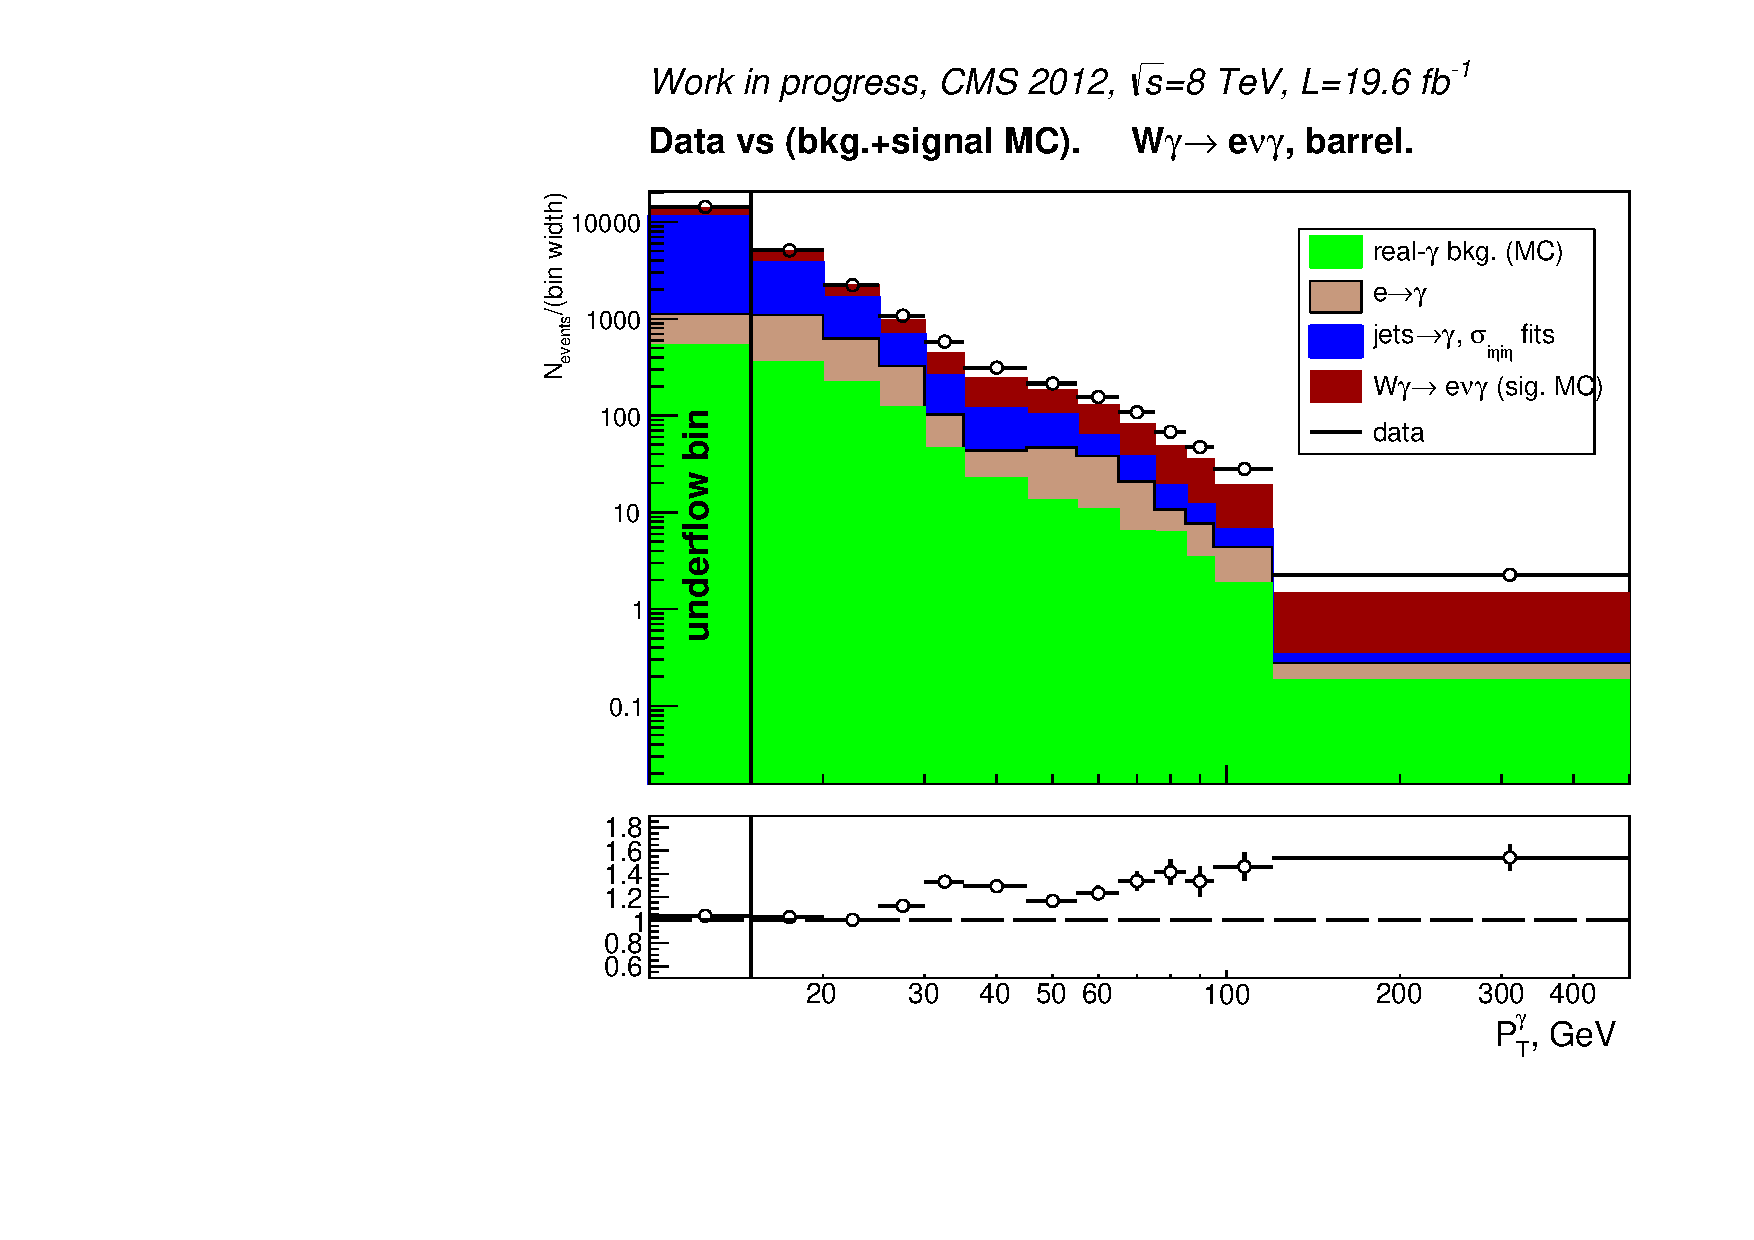
\includegraphics[width=0.45\textwidth]{../figs/figs_v11/ELECTRON_WGamma/PrepareYields/c_DATAvsBkgPlusSigMCc_ELECTRON_WGamma_TEMPL_SIHIH_UNblind__Barrel__phoEt.pdf}  \\
   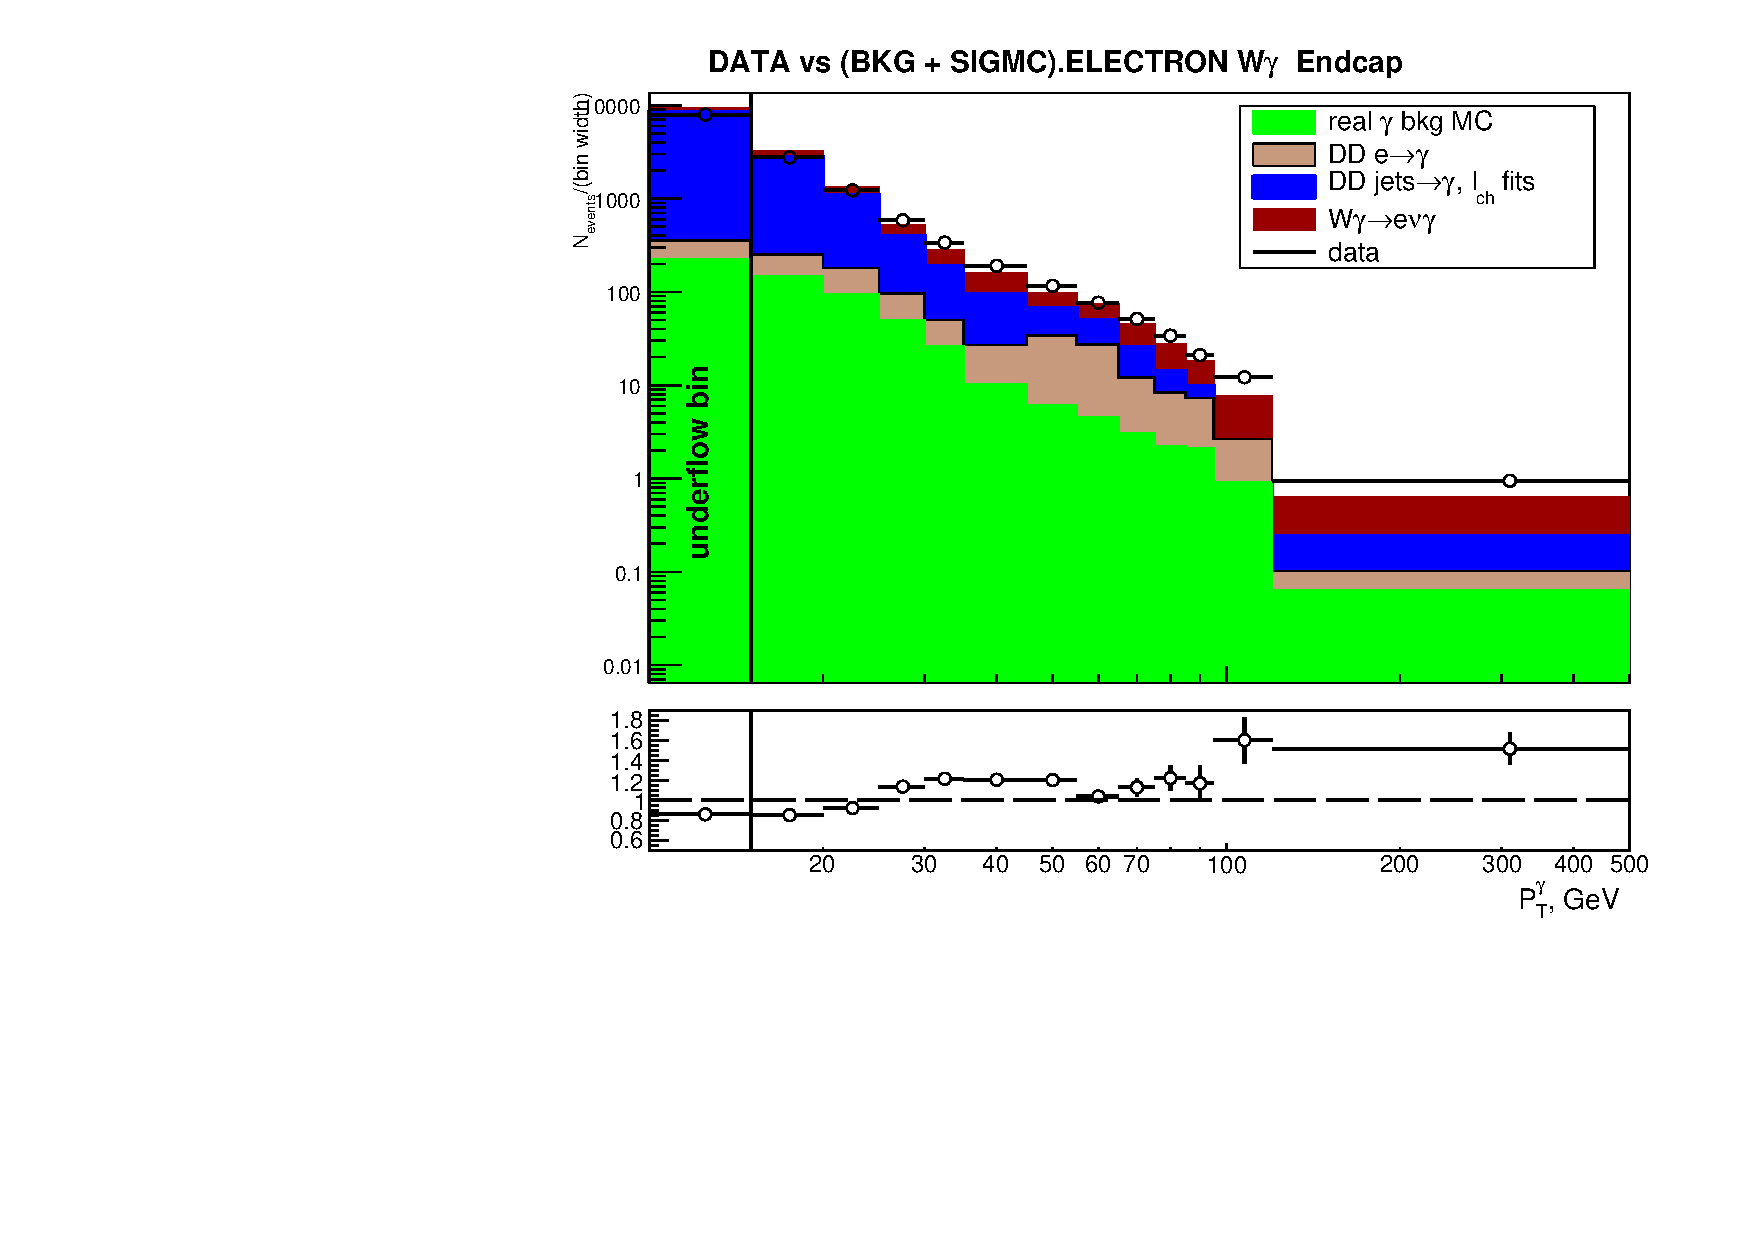
\includegraphics[width=0.45\textwidth]{../figs/figs_v11/ELECTRON_WGamma/PrepareYields/c_DATAvsBkgPlusSigMCc_ELECTRON_WGamma_TEMPL_CHISO_UNblind__Endcap__phoEt.pdf}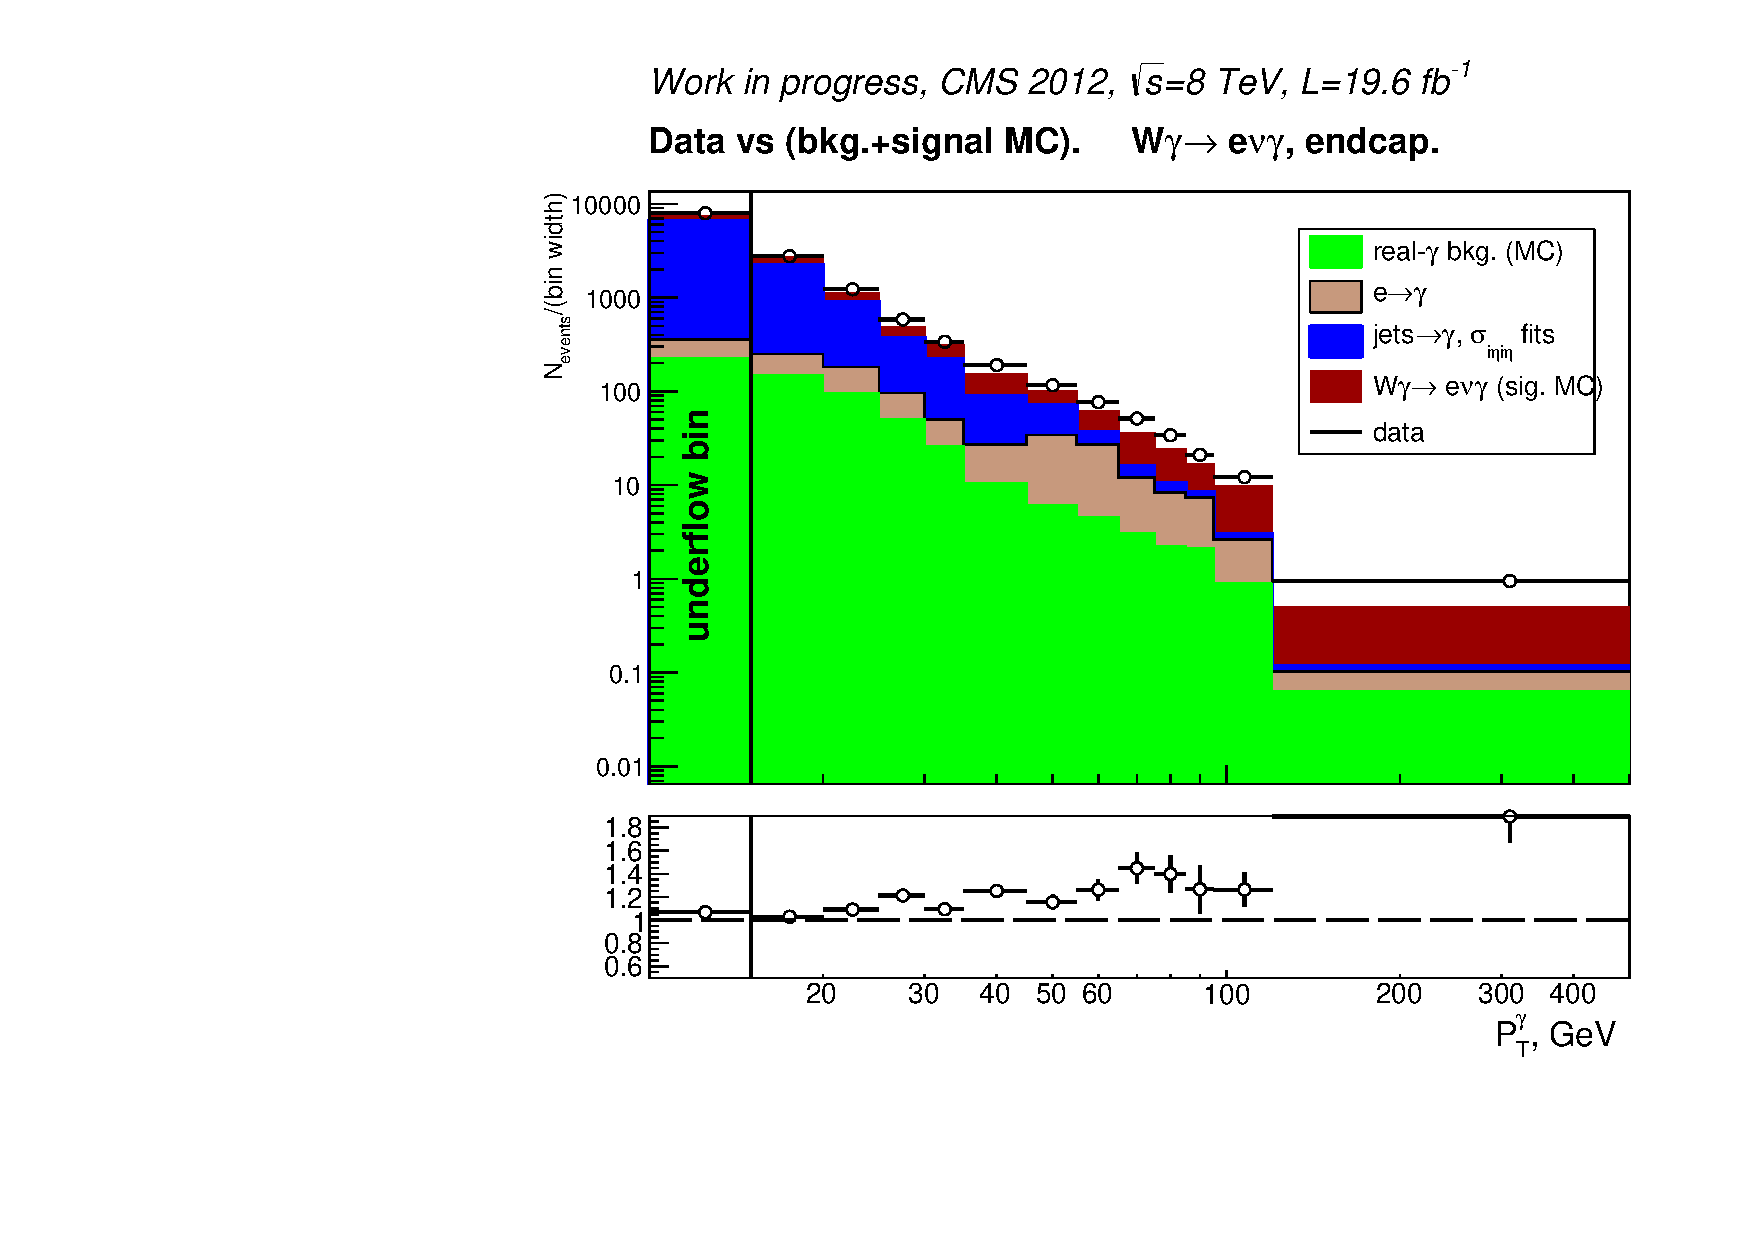
\includegraphics[width=0.45\textwidth]{../figs/figs_v11/ELECTRON_WGamma/PrepareYields/c_DATAvsBkgPlusSigMCc_ELECTRON_WGamma_TEMPL_SIHIH_UNblind__Endcap__phoEt.pdf}  \\
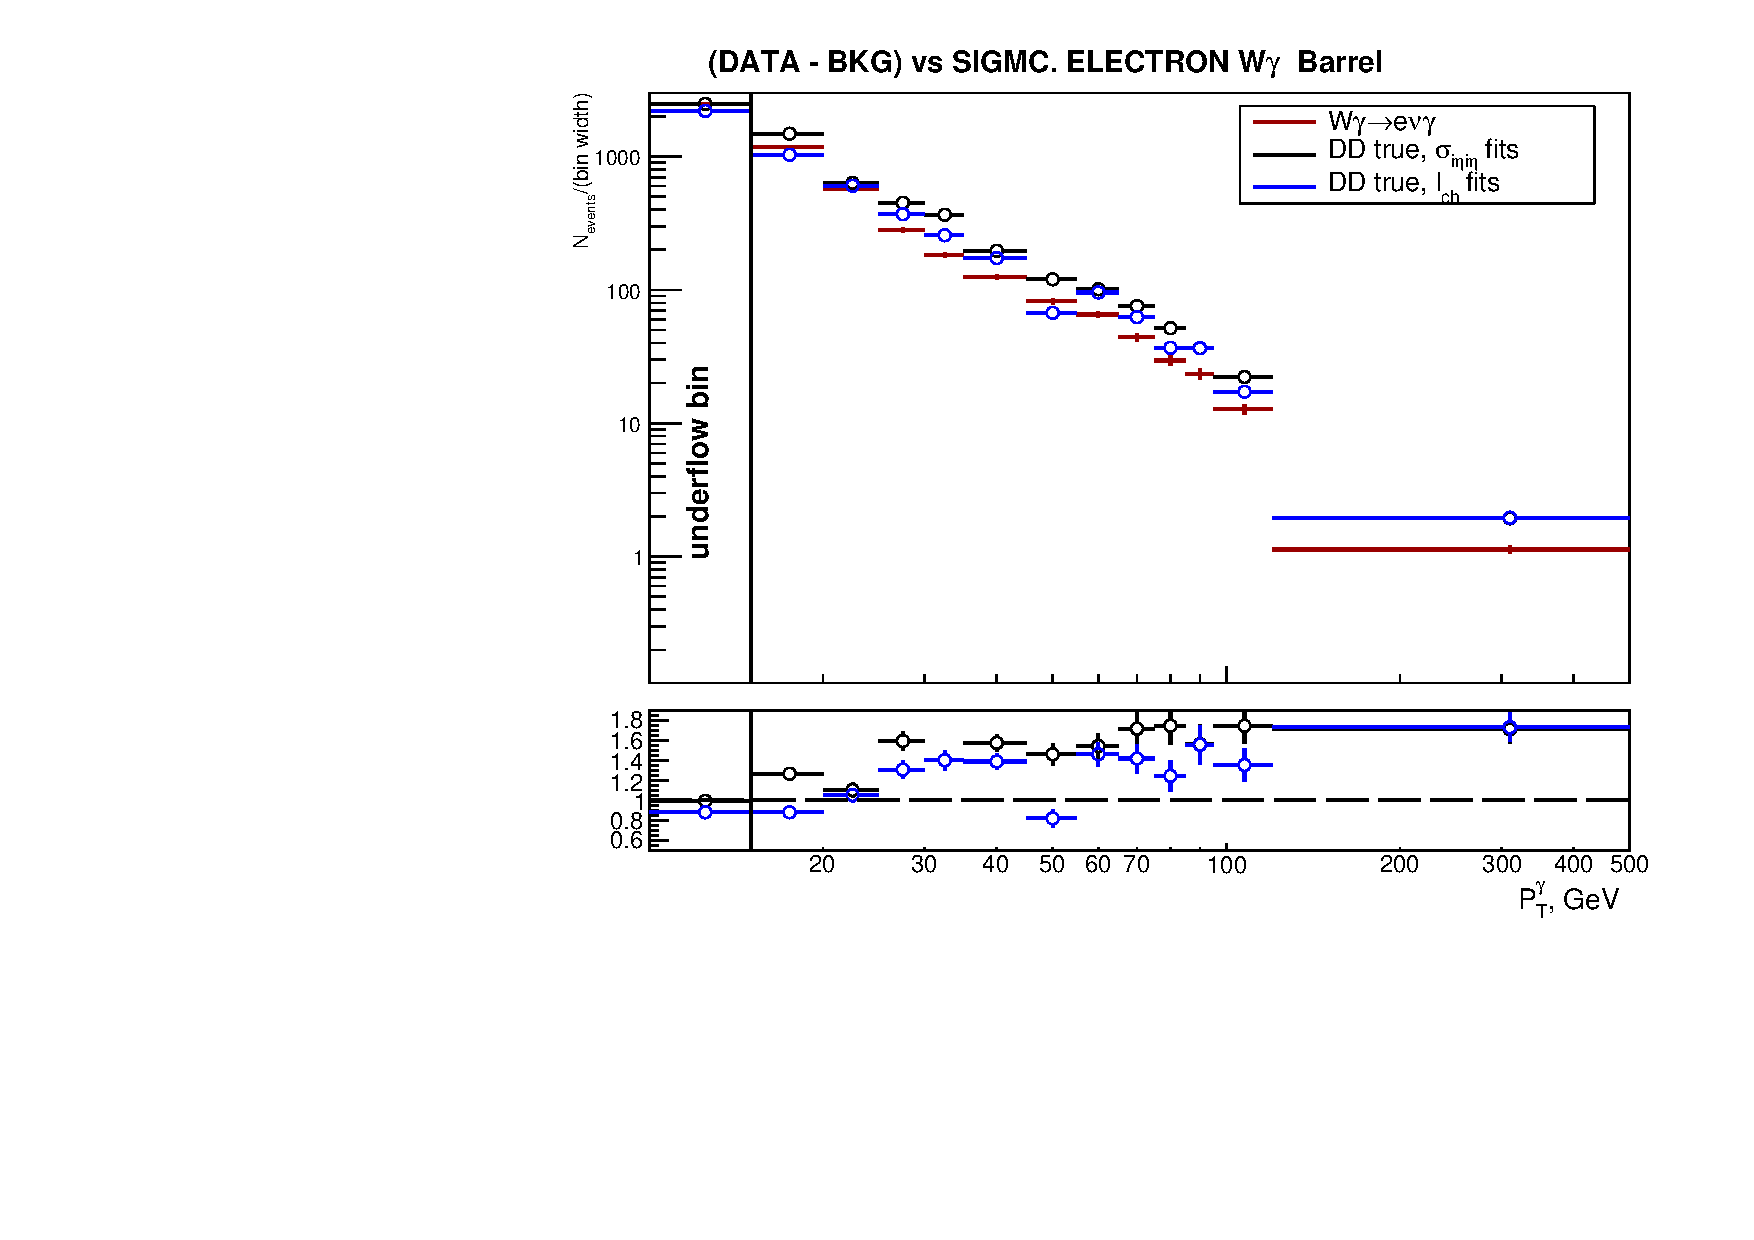
\includegraphics[width=0.45\textwidth]{../figs/figs_v11/ELECTRON_WGamma/PrepareYields/c_BkgSubtrDATAvsSIGMC_c_ELECTRON_WGamma__UNblind__Barrel__phoEt.pdf}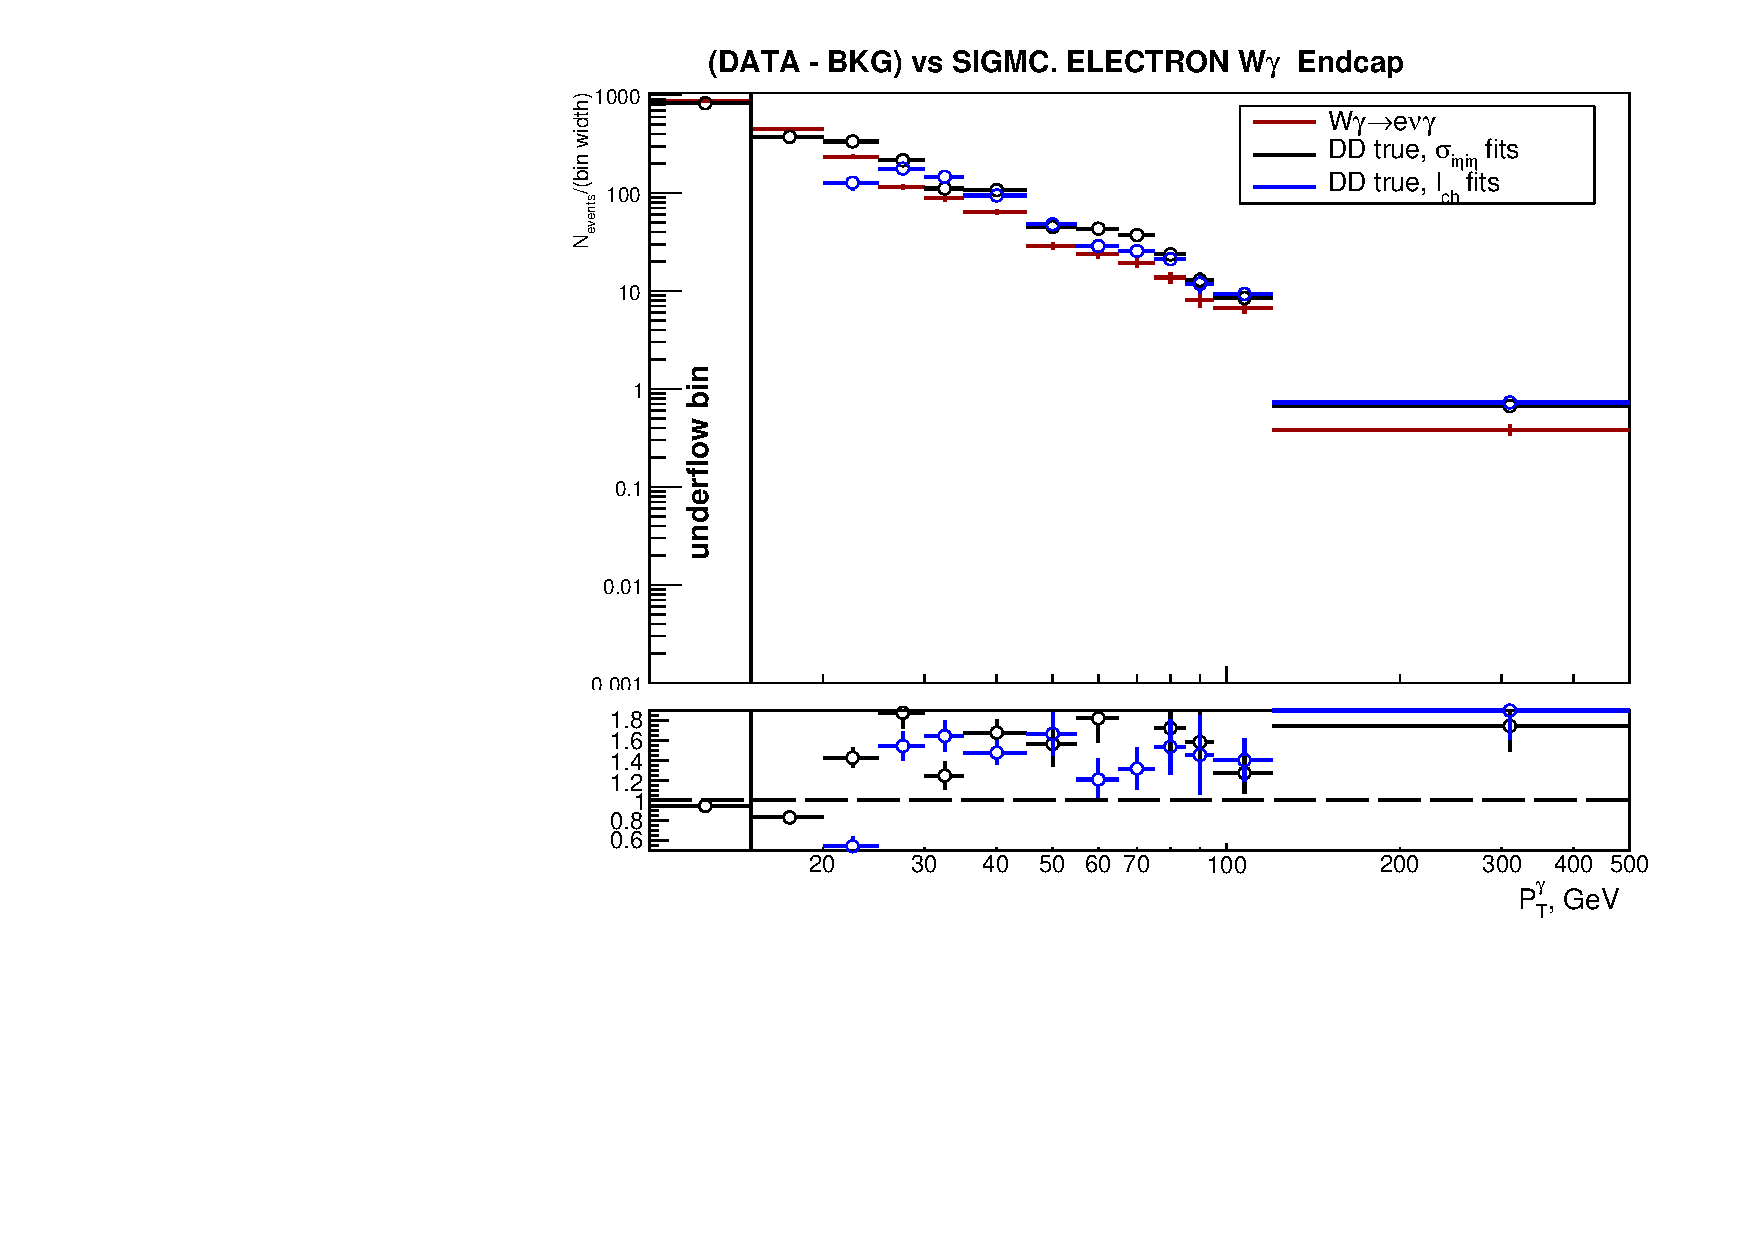
\includegraphics[width=0.45\textwidth]{../figs/figs_v11/ELECTRON_WGamma/PrepareYields/c_BkgSubtrDATAvsSIGMC_c_ELECTRON_WGamma__UNblind__Endcap__phoEt.pdf}\\
  \caption{Top and middle: data vs fake-$\gamma$ background derived from the template method + real-$\gamma$ background predicted by dedicated MC samples + signal MC, with $I_{ch}$ and $\sigma_{i\etai\eta}$ used as fit variables. Bottom: data yields after full background subtraction vs signal MC. $I_{ch}$ vs $\sigma_{i\etai\eta}$ fit results. }
  \label{fig:DDvsMC_Wg_Data_ELECTRON}
  \end{center}
\end{figure}

\begin{table}[h]
  \tiny
  \begin{center}
  \caption{Data, signal and background yields. WGamma MUON Barrel}
  \begin{tabular}{|c|c|c|c|c|c|c|c|}
    bin & DD fake & DD fake & MC real-\gamma & SIGMC & bkg+sig &  bkg+sig & data \\ 
    lims & CHISO & SIHIH & bkg & ($W\gamma\rightarrow\mu\nu\gamma$) & CHISO &  SIHIH &\\ \hline
 10-15 & 79833$\pm$251 & 77612$\pm$322 & 2549$\pm$46 & 26251$\pm$240 & 108633$\pm$350 & 106412$\pm$404 & 114047$\pm$338 \\ \hline 
15-20 & 21434$\pm$150 & 24543$\pm$143 & 1632$\pm$34 & 12707$\pm$164 & 35772$\pm$225 & 38882$\pm$221 & 41411$\pm$203 \\ \hline 
20-25 & 8466$\pm$101 & 9878$\pm$78 & 1331$\pm$31 & 6793$\pm$120 & 16590$\pm$160 & 18003$\pm$146 & 19801$\pm$141 \\ \hline 
25-30 & 3509$\pm$68 & 4402$\pm$46 & 1218$\pm$27 & 4087$\pm$93 & 8814$\pm$119 & 9708$\pm$107 & 11409$\pm$107 \\ \hline 
30-35 & 1687$\pm$49 & 2944$\pm$40 & 1282$\pm$28 & 2604$\pm$75 & 5572$\pm$93 & 6830$\pm$89 & 7717$\pm$88 \\ \hline 
35-45 & 1947$\pm$56 & 2540$\pm$33 & 1883$\pm$33 & 2971$\pm$80 & 6801$\pm$103 & 7393$\pm$93 & 9339$\pm$97 \\ \hline 
45-55 & 731$\pm$40 & 1964$\pm$40 & 507$\pm$18 & 1861$\pm$63 & 3100$\pm$77 & 4332$\pm$77 & 3950$\pm$63 \\ \hline 
55-65 & 415$\pm$25 & 363$\pm$11 & 186$\pm$12 & 1135$\pm$50 & 1737$\pm$57 & 1684$\pm$52 & 2172$\pm$47 \\ \hline 
65-75 & 177$\pm$17 & 466$\pm$19 & 96$\pm$8 & 664$\pm$38 & 937$\pm$42 & 1226$\pm$43 & 1320$\pm$36 \\ \hline 
75-85 & 103$\pm$13 & 238$\pm$16 & 62$\pm$7 & 452$\pm$31 & 616$\pm$34 & 751$\pm$36 & 899$\pm$30 \\ \hline 
85-95 & 76$\pm$11 & 146$\pm$11 & 43$\pm$7 & 341$\pm$27 & 459$\pm$30 & 530$\pm$30 & 600$\pm$24 \\ \hline 
95-120 & 67$\pm$11 & 319$\pm$25 & 76$\pm$9 & 454$\pm$31 & 597$\pm$34 & 849$\pm$41 & 856$\pm$29 \\ \hline 
120-500 & 28$\pm$7 & 83$\pm$7 & 82$\pm$8 & 547$\pm$34 & 656$\pm$36 & 711$\pm$36 & 897$\pm$30 \\ \hline 
  \end{tabular}
  \label{tab:yields_Wg_to_munu__Barrel_}
  \end{center}
\end{table}

\begin{table}[h]
  \tiny
  \begin{center}
  \caption{Data, signal and background yields. WGamma MUON Endcap}
  \begin{tabular}{|c|c|c|c|c|c|c|c|}
    bin & DD fake & DD fake & MC real-\gamma & SIGMC & bkg+sig &  bkg+sig & data \\ 
    lims & CHISO & SIHIH & bkg & ($W\gamma\rightarrow\mu\nu\gamma$) & CHISO &  SIHIH &\\ \hline
10-15 & 77649$\pm$215 & 81161$\pm$426 & 2675$\pm$41 & 10823$\pm$154 & 91148$\pm$268 & 94660$\pm$455 & 94370$\pm$307 \\ \hline 
15-20 & 25902$\pm$142 & 27661$\pm$184 & 1871$\pm$34 & 6474$\pm$120 & 34248$\pm$189 & 36006$\pm$222 & 34643$\pm$186 \\ \hline 
20-25 & 10018$\pm$93 & 11659$\pm$102 & 1319$\pm$29 & 3377$\pm$86 & 14714$\pm$130 & 16355$\pm$136 & 15988$\pm$126 \\ \hline 
25-30 & 4061$\pm$58 & 4558$\pm$51 & 888$\pm$23 & 2068$\pm$67 & 7017$\pm$92 & 7514$\pm$88 & 8429$\pm$92 \\ \hline 
30-35 & 2669$\pm$54 & 2268$\pm$32 & 654$\pm$19 & 1404$\pm$56 & 4727$\pm$80 & 4326$\pm$67 & 5110$\pm$71 \\ \hline 
35-45 & 1807$\pm$44 & 2113$\pm$29 & 791$\pm$22 & 1489$\pm$57 & 4087$\pm$76 & 4393$\pm$68 & 5414$\pm$74 \\ \hline 
45-55 & 1025$\pm$50 & 936$\pm$19 & 233$\pm$13 & 819$\pm$43 & 2077$\pm$67 & 1987$\pm$48 & 2422$\pm$49 \\ \hline 
55-65 & 270$\pm$19 & 564$\pm$16 & 103$\pm$9 & 551$\pm$35 & 924$\pm$41 & 1217$\pm$39 & 1217$\pm$35 \\ \hline 
65-75 & 87$\pm$11 & 346$\pm$13 & 59$\pm$7 & 280$\pm$25 & 426$\pm$28 & 685$\pm$29 & 703$\pm$27 \\ \hline 
75-85 & 63$\pm$9 & 117$\pm$6 & 35$\pm$5 & 186$\pm$20 & 284$\pm$23 & 338$\pm$22 & 451$\pm$21 \\ \hline 
85-95 & 37$\pm$7 & 56$\pm$4 & 24$\pm$5 & 139$\pm$18 & 201$\pm$20 & 220$\pm$19 & 303$\pm$17 \\ \hline 
95-120 & 20$\pm$5 & -81$\pm$5 & 38$\pm$6 & 209$\pm$22 & 267$\pm$23 & 166$\pm$23 & 433$\pm$21 \\ \hline 
120-500 & 11$\pm$4 & 153$\pm$12 & 18$\pm$2 & 157$\pm$19 & 186$\pm$19 & 327$\pm$22 & 396$\pm$20 \\ \hline 
  \end{tabular}
  \label{tab:yields_Wg_to_munu__Endcap_}
  \end{center}
\end{table}

\begin{table}[h]
  \tiny
  \begin{center}
  \caption{Data, signal and background yields. WGamma ELECTRON Barrel}
  \begin{tabular}{|c|c|c|c|c|c|c|c|c|}
    bin & DD fake & DD fake & DD & MC real-\gamma &  SIGMC & bkg+sig &  bkg+sig & data \\ 
    lims & CHISO & SIHIH &e\rightarrow\gamma & bkg & ($W\gamma\rightarrow\e\nu\gamma$) & CHISO &  SIHIH &\\ \hline
10-15 & 51004$\pm$200 & 53577$\pm$266 & 2923$\pm$80 & 2688$\pm$41 & 12480$\pm$164 & 69094$\pm$273 & 71668$\pm$325 & 71649$\pm$268 \\ \hline 
15-20 & 13487$\pm$118 & 14474$\pm$110 & 3715$\pm$178 & 1779$\pm$32 & 5858$\pm$110 & 24839$\pm$242 & 25826$\pm$238 & 25455$\pm$160 \\ \hline 
20-25 & 5112$\pm$78 & 4846$\pm$55 & 2023$\pm$137 & 1101$\pm$25 & 2869$\pm$77 & 11104$\pm$177 & 10839$\pm$168 & 11130$\pm$105 \\ \hline 
25-30 & 1748$\pm$47 & 1790$\pm$29 & 1031$\pm$72 & 603$\pm$18 & 1412$\pm$54 & 4794$\pm$103 & 4836$\pm$96 & 5388$\pm$73 \\ \hline 
30-35 & 752$\pm$32 & 1079$\pm$24 & 286$\pm$33 & 229$\pm$12 & 916$\pm$44 & 2182$\pm$65 & 2510$\pm$61 & 2907$\pm$54 \\ \hline 
35-45 & 735$\pm$34 & 1003$\pm$21 & 215$\pm$27 & 223$\pm$12 & 1248$\pm$51 & 2421$\pm$69 & 2689$\pm$63 & 3128$\pm$56 \\ \hline 
45-55 & 551$\pm$31 & 964$\pm$28 & 335$\pm$37 & 134$\pm$10 & 821$\pm$42 & 1842$\pm$65 & 2255$\pm$63 & 2147$\pm$46 \\ \hline 
55-65 & 228$\pm$19 & 211$\pm$8 & 272$\pm$39 & 108$\pm$9 & 654$\pm$37 & 1263$\pm$58 & 1246$\pm$55 & 1556$\pm$39 \\ \hline 
65-75 & 163$\pm$16 & 300$\pm$15 & 143$\pm$27 & 64$\pm$7 & 441$\pm$31 & 811$\pm$45 & 948$\pm$45 & 1083$\pm$33 \\ \hline 
75-85 & 79$\pm$11 & 224$\pm$15 & 45$\pm$13 & 62$\pm$7 & 295$\pm$26 & 481$\pm$31 & 626$\pm$33 & 680$\pm$26 \\ \hline 
85-95 & 43$\pm$9 & 99$\pm$9 & 43$\pm$17 & 34$\pm$5 & 234$\pm$23 & 354$\pm$30 & 411$\pm$30 & 473$\pm$22 \\ \hline 
95-120 & 53$\pm$9 & 274$\pm$24 & 63$\pm$19 & 47$\pm$5 & 318$\pm$27 & 481$\pm$34 & 702$\pm$41 & 703$\pm$27 \\ \hline 
120-500 & 23$\pm$6 & 61$\pm$6 & 34$\pm$12 & 71$\pm$8 & 430$\pm$31 & 558$\pm$35 & 595$\pm$35 & 859$\pm$29 \\ \hline 
  \end{tabular}
  \label{tab:systInPercentyields_Wg_to_enu__Barrel_}
  \end{center}
\end{table}

\begin{table}[h]
  \tiny
  \begin{center}
  \caption{Data, signal and background yields. WGamma ELECTRON Endcap}
  \begin{tabular}{|c|c|c|c|c|c|c|c|c|}
    bin & DD fake & DD fake & DD & MC real-\gamma &  SIGMC & bkg+sig &  bkg+sig & data \\ 
    lims & CHISO & SIHIH &e\rightarrow\gamma & bkg & ($W\gamma\rightarrow\e\nu\gamma$) & CHISO &  SIHIH &\\ \hline
 10-15 & 31043$\pm$138 & 40022$\pm$13 & 666$\pm$38 & 1120$\pm$27 & 4368$\pm$97 & 37197$\pm$174 & 46176$\pm$108 & 39746$\pm$199 \\ \hline 
15-20 & 9920$\pm$88 & 12692$\pm$124 & 509$\pm$56 & 744$\pm$21 & 2253$\pm$68 & 13426$\pm$127 & 16198$\pm$154 & 13818$\pm$118 \\ \hline 
20-25 & 3538$\pm$56 & 4558$\pm$63 & 433$\pm$36 & 473$\pm$17 & 1177$\pm$49 & 5621$\pm$84 & 6641$\pm$90 & 6133$\pm$78 \\ \hline 
25-30 & 1358$\pm$34 & 1516$\pm$29 & 229$\pm$24 & 250$\pm$12 & 575$\pm$34 & 2412$\pm$55 & 2569$\pm$52 & 2924$\pm$54 \\ \hline 
30-35 & 850$\pm$31 & 694$\pm$18 & 120$\pm$16 & 130$\pm$9 & 445$\pm$31 & 1546$\pm$48 & 1390$\pm$41 & 1690$\pm$41 \\ \hline 
35-45 & 613$\pm$26 & 670$\pm$16 & 167$\pm$19 & 103$\pm$8 & 638$\pm$37 & 1522$\pm$50 & 1578$\pm$46 & 1905$\pm$44 \\ \hline 
45-55 & 377$\pm$30 & 337$\pm$11 & 281$\pm$28 & 61$\pm$6 & 287$\pm$24 & 1006$\pm$49 & 965$\pm$40 & 1162$\pm$34 \\ \hline 
55-65 & 98$\pm$12 & 228$\pm$11 & 227$\pm$28 & 46$\pm$6 & 238$\pm$22 & 608$\pm$38 & 738$\pm$38 & 767$\pm$28 \\ \hline 
65-75 & 40$\pm$8 & 139$\pm$9 & 90$\pm$18 & 31$\pm$4 & 194$\pm$21 & 354$\pm$29 & 454$\pm$29 & 513$\pm$23 \\ \hline 
75-85 & 22$\pm$6 & 57$\pm$5 & 62$\pm$15 & 22$\pm$5 & 137$\pm$18 & 243$\pm$25 & 278$\pm$25 & 340$\pm$18 \\ \hline 
85-95 & 11$\pm$4 & 25$\pm$3 & 52$\pm$19 & 21$\pm$3 & 81$\pm$14 & 166$\pm$24 & 179$\pm$24 & 210$\pm$14 \\ \hline 
95-120 & 8$\pm$3 & -43$\pm$4 & 43$\pm$13 & 23$\pm$5 & 166$\pm$20 & 241$\pm$25 & 190$\pm$25 & 304$\pm$17 \\ \hline 
120-500 & 5$\pm$3 & 53$\pm$7 & 15$\pm$7 & 24$\pm$4 & 146$\pm$19 & 190$\pm$21 & 237$\pm$22 & 360$\pm$19 \\ \hline 
  \end{tabular}
  \label{tab:systInPercentyields_Wg_to_enu__Endcap_}
  \end{center}
\end{table}
